\chapter{Finite State Machines \label{chapter:finite-state-machines}} 

\begin{figure}[h] 
\centering
  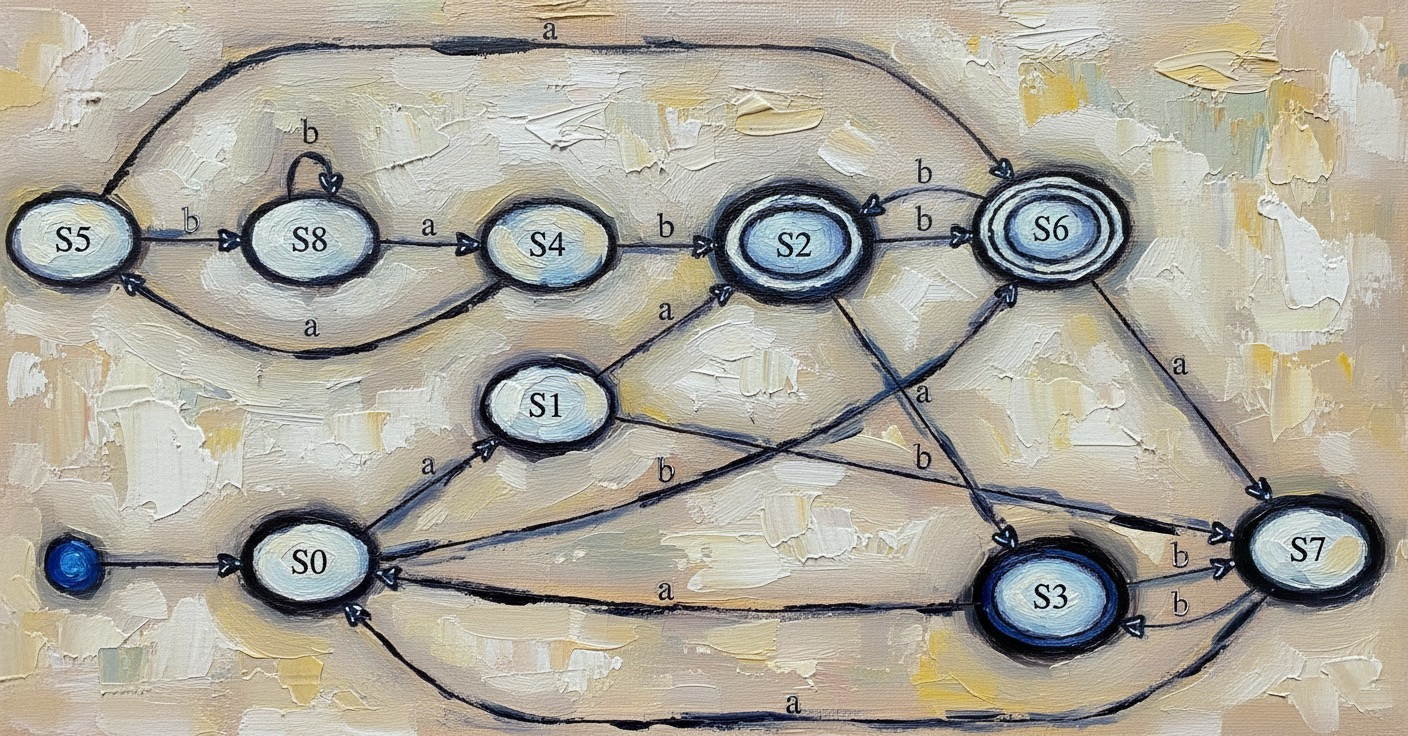
\includegraphics[width=12.5cm]{Abbildungen/finite-state-machine.jpg}
\caption{A finite state machine.}
\label{fig:finite-state-machine.png}
\end{figure}

\noindent
In the previous chapter we have seen how we can generate scanners from regular expressions.  In this chapter
we learn how regular expressions can be implemented using \blue{finite state machines}\index{finite state machine}.
In the literature, finite state machines are also called \blue{finite automata}\index{finite automaton}.  There are
two kinds of finite state machines: the \blue{deterministic finite automata}, abbreviated as \simtextsc{Dfa}s, and
the \blue{non-deterministic finite automata}\index{non-deterministic finite automaton}, abbreviated as
\simtextsc{Nfa}s.  Although \simtextsc{Nfa}s seem to be more powerful than \simtextsc{Dfa}s, we will see that every
\simtextsc{Nfa} can be transformed into an equivalent \simtextsc{Dfa}.  After proving this result, we show how a
regular expression can be translated into an equivalent \simtextsc{Nfa}.  Then we show that the language recognized
by any \simtextsc{Dfa} can be described by an equivalent regular expression.  Therefore, the central result of this
chapter is the equivalence of finite state machines and regular expressions.  Finally, we show how the number of
states of a \simtextsc{Dfa} can be minimized.  In detail, the results proved in this chapter are as follows:
\begin{enumerate}[(a)]
\item The language described by a regular expression can be defined by an \simtextsc{Nfa}.
\item Every \simtextsc{Nfa} can be transformed into an equivalent \simtextsc{Dfa}.
\item For every \simtextsc{Dfa} there is a regular expression specifying the language recognized by
      this \simtextsc{Dfa}.
\item For every \simtextsc{Dfa} there is an equivalent \simtextsc{Dfa} that has the minimal number of states.
\end{enumerate}


\section{Deterministic Finite Automata}
The finite state machines that we are going to discuss in this chapter are used to read a string and
to decide whether this string is an element of a given language.  Hence, the input of these 
\simtextsc{Dfa}s is a string, while the output is either the value \texttt{True} or the value \texttt{False}.
The name-giving feature of a \simtextsc{Dfa} is the fact that a \simtextsc{Dfa} only has a
\underline{finite} number of possible states.  Reading a character causes the \simtextsc{Dfa} to change its state.
A \simtextsc{Dfa} accepts its input if it has reached a so-called \blue{accepting state} after reading
all characters of the input string.  Let me explain this idea more precisely:
\begin{enumerate}[(a)]
\item Initially, the \simtextsc{Dfa} is in a state that is known as the \blue{start state}. \index{start state}
\item In every step of its computation, the \simtextsc{Dfa} reads one character of the input string
      $s$.  Every time a character is processed, the state of the \simtextsc{Dfa} might change.
\item Some states of the \simtextsc{Dfa} are designated as \blue{accepting states}.  \index{accepting state}
      If the \simtextsc{Dfa} has consumed all characters of the given input string $s$ and the \simtextsc{Dfa}
      has reached an accepting state, then the input string $s$ is accepted and the \simtextsc{Dfa}
      returns \texttt{True}.  Otherwise the \simtextsc{Dfa} returns \texttt{False} and the string $s$
      is rejected.
\end{enumerate}
\begin{figure}[!ht]
  \centering
      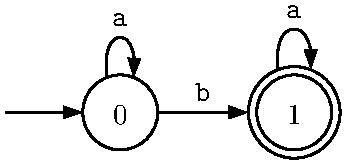
\includegraphics[scale=0.8]{Abbildungen/abstara.pdf}
   \caption{A \simtextsc{Dfa} to recognize the language $L(\texttt{a}^*\cdot\texttt{b}\cdot\texttt{a}^*)$.}
  \label{fig:abstara.dot}
\end{figure}


\noindent
Finite state machines are best presented graphically.  Figure \ref{fig:abstara.dot} depicts a simple
\simtextsc{Dfa} that recognizes those strings that are specified by the regular expression
\\[0.2cm]
\hspace*{1.3cm}
$\texttt{a}^*\cdot\texttt{b}\cdot\texttt{a}^*$.
\\[0.2cm]
This \simtextsc{Dfa} has but two states.  These states are called $0$ and $1$.
\begin{enumerate}
\item State $0$  is the start state.  In Figure \ref{fig:abstara.dot}, the start state is indicated by an arrow
      coming from the left that points to it.  
  
      If the \simtextsc{Dfa} is in the state $0$ and reads the character ``\texttt{a}'', then the
      \simtextsc{Dfa} stays in the state $0$.  This is specified in the figure by an arrow labeled with the
      character ``\texttt{a}'' that both starts and ends in the state $0$.  On the other hand, if the
      character ``\texttt{b}'' is read while the \simtextsc{Dfa} is in state 0, then the \simtextsc{Dfa}
      switches into the state $1$.  This is depicted by an arrow labeled with the character
      ``\texttt{b}'' that originates from the state $0$ and points to the state $1$.
\item State  $1$ is an accepting state. In Figure \ref{fig:abstara.dot} this is specified by the
      fact that the state $1$ is decorated by a double circle.

      If the character ``\texttt{a}'' is read while the \simtextsc{Dfa} is in state $1$, then the
      \simtextsc{Dfa} does not change its state.  On the other hand, if the \simtextsc{Dfa} reads the
      character ``\texttt{b}'' while in state $1$, then the next state is undefined since there is no
      arrow originating from state $1$ that is labeled with the character ``\texttt{b}''.

      In general, a \simtextsc{Dfa} \blue{dies} \index{death of a \simtextsc{Dfa}}
      if it reads a character $c$ in a state $s$ such that there is no transition from $s$ when $c$ is read.
      In this case, the \simtextsc{Dfa} does not accept the given input string.
\end{enumerate}

\noindent
Formally, a \href{http://en.wikipedia.org/wiki/Finite-state_machine}{\emph{deterministic finite automaton}} 
\index{deterministic finite automaton}
is defined as a 5-tuple.
\begin{Definition}[\simtextsc{Dfa}]
A \blue{deterministic finite automaton} (abbreviated as \simtextsc{Dfa}\index{DFA@\simtextsc{Dfa}}\glsadd{dfa}) is a 5-tuple 
\\[0.2cm]
\hspace*{1.3cm}
$F = \langle Q, \Sigma, \delta, q_0, A\rangle$
\\[0.2cm]
where the components $Q$, $\Sigma$, $\delta$, $q_0$, and $A$ have the following properties:
\begin{enumerate}
\item $Q$ is the \underline{finite} \blue{set of states}.
\item $\Sigma$ is the \blue{input alphabet}\index{input alphabet}\index{$\Sigma$}.  Therefore, $\Sigma$ is a
      set of characters and 
      the strings read by the \simtextsc{Dfa} $F$ are strings from the set $\Sigma^*$.
\item $\delta: Q \times \Sigma \rightarrow Q \cup \{ \Omega \}$\glsadd{omega}

      is the  \blue{transition function}\index{transition function}.  For every state $q\in Q$ and for all
      characters $c \in \Sigma$ the expression $\delta(q,c)$ computes the new state of the \simtextsc{Dfa} $F$
      that is reached if $F$ reads the character $c$ while in state $q$.
      If $\delta(q,c) = \Omega$, then $F$ \blue{dies} when it is in state $q$ and the next character
      is $c$. 

      In the figures depicting \simtextsc{Dfa}s transitions of the form $\delta(q, c) = \Omega$ 
      are not shown.
\item $q_0 \in Q$ is the \blue{start state}. \index{start state}
\item $A \subseteq Q$ is the set of \blue{accepting states}. \index{accepting state}
      \eox
\end{enumerate}
\end{Definition}

\exampleEng
The \simtextsc{Dfa} that is shown in Figure  \ref{fig:abstara.dot} is formally defined as follows:
\\[0.2cm]
\hspace*{1.3cm}
$F = \langle Q, \Sigma, \delta, q_0, A \rangle$,
\\[0.2cm]
where we have:
\begin{enumerate}
\item $Q = \{ 0, 1 \}$,
\item $\Sigma = \{ \texttt{a}, \texttt{b} \}$,
\item $\delta = \bigl\{ 
                        \pair(0,a) \mapsto 0, 
                        \pair(0,b) \mapsto 1, 
                        \pair(1,a) \mapsto 1, 
                        \pair(1,b) \mapsto \Omega 
                \bigr\}$,
\item $q_0 = 0$,
\item $A = \{ 1 \}$.
\end{enumerate}
In order to formally define the language $L(F)$ that is accepted by a \simtextsc{Dfa} $F$
we generalize the transition function $\delta$ to a new function
\\[0.2cm]
\hspace*{1.3cm}
$\delta^*: Q \times \Sigma^* \rightarrow Q \cup \{ \Omega \}$\glsadd{deltastar}
\\[0.2cm]
that, instead of a single character, accepts a string as its second argument.  The definition of
$\delta^*(q, w)$ is given by induction on the string $w$.
\begin{enumerate}
\item[I.A.] $w = \lambda$:  We define
            \\[0.2cm]
            \hspace*{1.3cm}
            $\delta^*(q, \lambda) := q$,
            \\[0.2cm]
            because if a \simtextsc{Dfa} does not read any character, it cannot change its state. 
\item[I.S.] $w = cv$ where $c \in \Sigma$ and $v  \in \Sigma^*$:  We define
            \\[0.2cm]
            \hspace*{1.3cm}
            $\delta^*(q, cv) := \left\{
            \begin{array}[c]{ll}              
            \delta^*\bigl(\delta(q,c),v\bigr) & \mbox{provided $\delta(q,c) \not= \Omega$;} \\
            \Omega                            & \mbox{otherwise}.
            \end{array}
            \right.
            $
            \\[0.2cm]
            If $F$ reads the string  $cv$, it first reads the character $c$.  Now if this causes  $F$
            to change into the state $\delta(q,c)$, then $F$ has to read the string $v$ in the state
            $\delta(q,c)$.  However, 
            if  $\delta(q,c)$ is undefined, then  $\delta^*(q,cv)$ is undefined too.
\end{enumerate}

\begin{Definition}[Accepted Language, $L(F)$]
  \index{accepted language} \index{$L(F)$}\glsadd{langoffsm}
  For a \simtextsc{Dfa} $F = \langle Q, \Sigma, \delta, q_0, A \rangle$ the \blue{language accepted by $F$} 
  is called $L(F)$ and is defined as
  \\[0.2cm]
  \hspace*{1.3cm}
  $L(F) := \bigl\{ s \in \Sigma^* \mid \delta^*(q_0,s) \in A \bigr\}$. 
  \\[0.2cm]
  Hence, the accepted language of $F$ is the set of all those strings that take $F$ from its
  start state into an accepting state. \eox
\end{Definition}

\exerciseEng
Specify a \simtextsc{Dfa} $F$ such that $L(F)$ is the set of all those strings $s \in \{a,b\}^*$, 
such that $s$ contains the substring  ``\texttt{aba}''.
\eox


\paragraph{Complete Finite State Machines}
Occasionally it is beneficial for a \simtextsc{Dfa} $F$ to be \blue{complete}: A \simtextsc{Dfa}
\\[0.2cm]
\hspace*{1.3cm}
$F = \langle Q, \Sigma, \delta, q_0, A \rangle$,
\\[0.2cm]
is \blue{complete}\index{complete, finite state machine} if the transition function $\delta$ never returns the
undefined value $\Omega$, i.e.~we have 
\\[0.2cm]
\hspace*{1.3cm}
$\delta(q, c) \not= \Omega$ \quad for all $q \in Q$ and $c \in \Sigma$.

\begin{Proposition}
  For every \simtextsc{Dfa} $F$ there exists a complete \simtextsc{Dfa}  $\widehat{F}$ that accepts
  the same language as the \simtextsc{Dfa}  $F$, i.e.~we have:
  \\[0.2cm]
  \hspace*{1.3cm}
  $L(\widehat{F}) = L(F)$.
\end{Proposition}

\proofEng
Assume $F$ is given as
\\[0.2cm]
\hspace*{1.3cm}
$F = \langle Q, \Sigma, \delta, q_0, A \rangle$.
\\[0.2cm]
The idea is to define $\widehat{F}$ by adding a new state to the set of states $Q$.  This new state is called
the  \blue{dead state}. \index{dead state} If there is no next state for a given state  $q \in Q$ when a character $c$
is processed, i.e.~if we have
\\[0.2cm]
\hspace*{1.3cm}
$\delta(q, c) = \Omega$,
\\[0.2cm]
then $F$ changes into the dead state.  Once $F$ has reached a dead state, it will never leave this
state.

The formal definition of the \simtextsc{Dfa} $\widehat{F}$ is done as follows:
We introduce a new state $\skull$ which serves as the \blue{dead state}.\glsadd{skull}  The only requirement is that $\skull \not\in Q$.
\begin{enumerate}
\item $\widehat{Q} := Q \cup \{ \skull \}$,

      the dead state is added to the set  $Q$.
\item $\widehat{\delta} : \widehat{Q} \times \Sigma \rightarrow \widehat{Q}$,

      where the function $\widehat{\delta}$ is defined as follows:
      \begin{enumerate}
      \item $\delta(q,c) \not= \Omega \rightarrow \widehat{\delta}(q,c) = \delta(q,c)$ \quad  for all $q \in Q$ and $c \in \Sigma$.

            If the state transition function is defined for the state  $q$ and the character
            $c$, then $\widehat{\delta}(q,c)$ is the same as $\delta(q,c)$.
      \item $\delta(q,c) = \Omega \rightarrow \widehat{\delta}(q,c) = \skull$  \quad for all $q \in Q$ and $c \in \Sigma$.

            If the state transition function $\delta$ is undefined for the state $q$ and the character
            $c$, then $\widehat{\delta}(q,c)$ returns the dead state $\skull$.
      \item $\widehat{\delta}(\skull, c) = \skull$ \quad for all $c \in \Sigma$,

            because there is no escape from death.
      \end{enumerate}
\end{enumerate}
Hence the \simtextsc{Dfa}  $\widehat{F}$ is given as follows:
\\[0.2cm]
\hspace*{1.3cm}
$\widehat{F} = \langle \widehat{Q}, \Sigma, \widehat{\delta}, q_0, A \rangle$.
\\[0.2cm]
If  $F$ reads a string $s$ without reaching an undefined state, then the behavior of $F$ and $\widehat{F}$ is the same.
However, if $F$ reaches an undefined state, then $\widehat{F}$ instead switches into the dead state 
$\skull$ and remains in this state regardless of the rest of the input string.  As the dead state $\skull$
is not an accepting state, the languages accepted by  $F$ and $\widehat{F}$ are identical. \qed 

\exerciseEng
Define a \simtextsc{Dfa} that accepts the language specified by the regular expression 
\\[0.2cm]
\hspace*{1.3cm}
$r := (\texttt{a}+\texttt{b})^* \cdot \texttt{b} \cdot (\texttt{a}+\texttt{b}) \cdot
(\texttt{a}+\texttt{b})$. \eox

\solutionEng
The regular expression $r$ specifies those strings $s$ from the alphabet 
$\Sigma = \{ \mathtt{a}, \mathtt{b} \}$ such that the antepenultimate character of $s$ is the
character ``\texttt{b}''.  In order to recognize this fact, the \simtextsc{Dfa} has to remember the
last three characters.  As there are eight different possible combinations for the last three
characters, the \simtextsc{Dfa} needs to have eight states.  Let us number these states 
 $0$, $1$, $2$, $\cdots$, $7$.  We describe the purpose of these states in the following:
\begin{description}
\item[State 0:] In this state, the character ``\texttt{b}'' has not yet been seen. 
  Depending on how many characters have been read, there are four cases:
  \begin{enumerate}[(a)]
  \item At least three characters have been read.  In this case, the last three characters are ``\texttt{aaa}''.  
  \item Two characters have been read.  In this case, the string that has been read so far is the string ``\texttt{aa}''.  
  \item Only one character has been read so far. In this case, the string that has been read is ``\texttt{a}''.  
  \item Nothing has yet been read and therefore the string that has been read is $\lambda$.
  \end{enumerate}

                For the remaining states we list the last three characters  that have been read
                without further comment.
\item[State 1:] ``\texttt{aab}''.

                This case also covers the cases where the strings ``\texttt{ab}'' and ``\texttt{b}''
                have been read.
\item[State 2:] ``\texttt{aba}''.

                This case also covers the case where the string ``\texttt{ba}''
                has been read.
\item[State 3:] ``\texttt{abb}''.

                This case also covers the case where the string ``\texttt{bb}''
                has been read.
\item[State 4:] ``\texttt{bab}''.
\item[State 5:] ``\texttt{bba}''.
\item[State 6:] ``\texttt{bbb}''.
\item[State 7:] ``\texttt{baa}''.
\end{description}
Obviously, the states 4, 5, 6 and 7 are the accepting states because here the antepenultimate
character is the character ``\texttt{b}''.  Next, we construct the transition function $\delta$.
\begin{enumerate}
\item[0.] First, let us consider the state 0.  If the last three characters that have been read are
          ``\texttt{aaa}'' and if we read the character ``\texttt{a}'' next, then the last three
          characters read will again be ``\texttt{aaa}''.  Hence, we must have
          \\[0.2cm]
          \hspace*{1.3cm}
          $\delta(0, \mathtt{a}) = 0$.
          \\[0.2cm]
          However, if instead we read the character ``\texttt{b}'' in state 0, then the last three
          characters that have been read are ``\texttt{aab}'', which is exactly the last three
          characters that have been read in state 1.  Hence we have
          \\[0.2cm]
          \hspace*{1.3cm}
          $\delta(0, \mathtt{b}) = 1$.
\item[1.] Next we consider state 1.  If the last three characters are ``\texttt{aab}'' and we read
          the character ``\texttt{a}'' next, then the last three characters are ``\texttt{aba}''.
          This corresponds to the state  2.  Therefore, we must have
          \\[0.2cm]
          \hspace*{1.3cm}
          $\delta(1, \mathtt{a}) = 2$.
          \\[0.2cm]
          If instead we read the character  ``\texttt{b}'' while in state 1, then the last three
          characters will be ``\texttt{abb}'', which corresponds to the state number  3.  Hence we have
          \\[0.2cm]
          \hspace*{1.3cm}
          $\delta(1, \mathtt{b}) = 3$.
\end{enumerate}
The remaining transitions are found in a similar way.
Figure \ref{fig:abstarbabab.dot} on page \pageref{fig:abstarbabab.dot} shows the resulting \simtextsc{Dfa}.
We still have to explain how we have chosen the start state.  When the computation starts, the
finite state machine has not read any character.  In particular, this implies that neither of the
last three characters is the character ``\texttt{b}''.   Hence we can use the state 0 as the start
state of our \simtextsc{Dfa}.

 \begin{figure}[!ht]
   \centering
       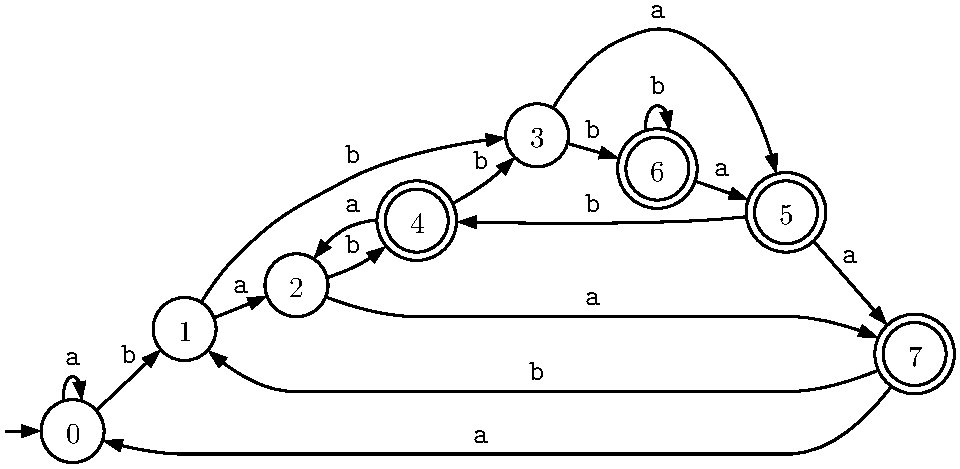
\includegraphics[scale=1.0]{Abbildungen/abstarbabab.pdf}
    \caption{A \simtextsc{Dfa} accepting
             $L\bigl((\texttt{a}+\texttt{b})^* \cdot \texttt{b} \cdot (\texttt{a}+\texttt{b}) \cdot (\texttt{a}+\texttt{b})\bigr)$.}
   \label{fig:abstarbabab.dot}
 \end{figure}

\remarkEng
There is a nice tool available that can be used to better understand finite state machines.  This
tool is available at
\\[0.2cm]
\hspace*{1.3cm}
\href{https://ivanzuzak.info/noam/webapps/fsm_simulator/}{\texttt{https://ivanzuzak.info/noam/webapps/fsm\_simulator/}}.


\section{Non-Deterministic Finite Automata}
For many applications, the \simtextsc{Dfa}s introduced in the previous section are unwieldy
because they have a large number of states.  For example, a \simtextsc{Dfa} that recognizes the language
\\[0.2cm]
\hspace*{1.3cm}
$L\bigl((\texttt{a}+\texttt{b})^* \cdot \texttt{b} \cdot (\texttt{a}+\texttt{b}) \cdot (\texttt{a}+\texttt{b})\bigr)$ 
\\[0.2cm]
needs 8 different states since the \simtextsc{Dfa} needs to remember the last three characters that
have been read and there are $2^3 = 8$ combinations of these characters.  
It would be possible to simplify this finite state machine if the machine would be permitted to \emph{choose} its
next state from a given set of states.

\begin{figure}[!ht]
  \centering
      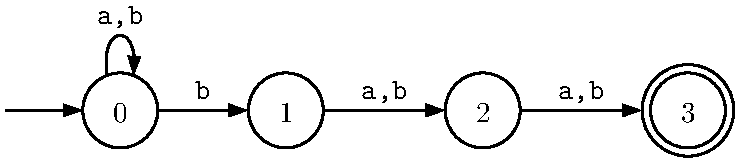
\includegraphics[scale=0.8]{Abbildungen/abstarbabab-nd.pdf}
   \caption{A non-deterministic finite automaton to recognize 
           $L\bigl((\texttt{a}+\texttt{b})^* \cdot \texttt{b} \cdot (\texttt{a}+\texttt{b}) \cdot (\texttt{a}+\texttt{b})\bigr)$.}
  \label{fig:abstarbabab-nd.dot}
\end{figure}
\noindent
Figure \ref{fig:abstarbabab-nd.dot} presents a \blue{non-deterministic finite automaton} (abbreviated as
\simtextsc{Nfa}) that accepts
the language specified by the regular expression
\\[0.2cm]
\hspace*{1.3cm}
$(\texttt{a}+\texttt{b})^* \cdot \texttt{b} \cdot (\texttt{a}+\texttt{b}) \cdot (\texttt{a}+\texttt{b})$.
\\[0.2cm]
This \simtextsc{Nfa} has only 4 different states that are named $0$, $1$, $2$ and $3$.
\begin{enumerate}
\item $0$ is the start state.  If the \simtextsc{Nfa} reads the letter ``\texttt{a}'' while it is in this
      state, the \simtextsc{Nfa} will stay in state $0$.  However, if the \simtextsc{Nfa} reads the
      character ``\texttt{b}'', then the \simtextsc{Nfa} has a \emph{choice}:  It can either stay in state
      $0$, or it might switch to the state $1$.
\item In state $1$ the \simtextsc{Nfa} switches to state $2$ if it reads either the character
      ``\texttt{a}'' or the character ``\texttt{b}''.
\item In state $2$ the \simtextsc{Nfa} switches to state $3$ if it reads either the character
      ``\texttt{a}'' or the character ``\texttt{b}''.
\item State  $3$ is the accepting state.  There is no transition from this state.  Hence, if the
      \simtextsc{Nfa} is in state 3 and there are still characters to read, then the \simtextsc{Nfa} dies.
\end{enumerate}
The finite state machine in Figure \ref{fig:abstarbabab-nd.dot} is non-deterministic because it has
to guess the next state if it is in state $0$ and reads the character ``\texttt{b}''.  Let us consider a possible
\emph{computation} of the \simtextsc{Nfa} when it reads the input ``\texttt{abab}'':
\\[0.2cm]
\hspace*{1.3cm}
$0 \comp{a} 0 \comp{b} 1 \comp{a} 2 \comp{b} 3$
\\[0.2cm]
In this computation, the \simtextsc{Nfa} has chosen the correct transition when reading the first
occurrence of the character ``\texttt{b}''.  If the \simtextsc{Nfa} had stayed in the state $0$ instead
of switching into the state 1, it would have been impossible to reach the accepting state 3 later
because then the computation would have worked out as follows:
\\[0.2cm]
\hspace*{1.3cm}
$0 \comp{a} 0 \comp{b} 0 \comp{a} 0 \comp{b} 1$
\\[0.2cm] 
Here, the \simtextsc{Nfa} is in state 1 after consuming the input string ``\texttt{abab}'' and as state
1 is not an accepting state, the \simtextsc{Nfa} would have falsely rejected the string ``\texttt{abab}''.
Let us consider a different example where the input is the string ``\texttt{bbbbb}'':
\\[0.2cm]
\hspace*{1.3cm}
$0 \comp{b} 0 \comp{b} 1 \comp{b} 2 \comp{b} 3 \comp{b} \Omega$
\\[0.2cm]
Here, the \simtextsc{Nfa} has switched too early into the state 1.  In this case, the \simtextsc{Nfa} dies
when reading the last character ``\texttt{b}''.  If the \simtextsc{Nfa} had stayed in state $0$ when reading the second
occurrence of the character ``\texttt{b}'', then it would have correctly accepted the string
``\texttt{bbbbb}'' since then the computation could have been as follows:
\\[0.2cm]
\hspace*{1.3cm}
$0 \comp{b} 0 \comp{b} 0 \comp{b} 1 \comp{b} 2 \comp{b} 3$.
\\[0.2cm]
The previous examples show that in order to avoid premature death, the given non-deterministic \simtextsc{Nfa} has
to choose its successor state
\href{https://www.youtube.com/watch?v=c3RN9zz77Cs}{wisely}.  
If $F$ is a non-deterministic \simtextsc{Nfa} and $s$ is a string such that $F$ can, when reading $s$,
choose its successor so that it reaches an accepting state after having read $s$, then the string
$s$ is an element of the language $L(F)$.

It seems that the concept of an \simtextsc{Nfa} is far more powerful than the 
concept of a \simtextsc{Dfa}.  After all, an \simtextsc{Nfa} appears to have some form of clairvoyance for else it
could not guess which states to choose.  However, we will prove in the 
next section that both \simtextsc{Dfa}s and \simtextsc{Nfa}s have the same power to
recognize languages:  Every language recognized by an \simtextsc{Nfa} is also
recognized by a \simtextsc{Dfa}.  In order to prove this claim, we have to
formalize the notion of an \simtextsc{Nfa}.  The definition that follows is more
general than the informal description of an \simtextsc{Nfa} given so far, as we will
allow the \simtextsc{Nfa} to also have \blue{$\varepsilon$-transitions}\index{epsilon-transition@$\varepsilon$-transition}.  An $\varepsilon$-transition
allows the \simtextsc{Nfa} to switch its state without reading any character.  For example, if there is
an $\varepsilon$-transition from the state 1 into the state 2, we write
\\[0.2cm]
\hspace*{1.3cm}
$1 \comp{\varepsilon} 2$.


\begin{Definition}[NFA]
A \blue{non-deterministic finite automaton}\index{non-deterministic finite automaton} \index{NFA@\simtextsc{Nfa}}
(abbreviated as \blue{\simtextsc{Nfa}}) 
is a  5-tuple
\\[0.2cm]
\hspace*{1.3cm}
$\langle Q, \Sigma, \delta, q_0, A\rangle$,
\\[0.2cm]
such that the following holds:
\begin{enumerate}
\item $Q$ is the finite \blue{set of states}.
\item $\Sigma$ is the \blue{input alphabet}.
\item $\delta$ is a function from $Q \times (\Sigma \cup \{ \varepsilon \})$ that assigns a set of states
      $\delta(q, a) \subseteq Q$ to every pair $\pair(q, a)$ from $Q \times (\Sigma \cup \{ \varepsilon \})$:
      \\[0.2cm]
      \hspace*{1.3cm}
      $\delta: Q \times (\Sigma \cup \{\varepsilon\}) \rightarrow 2^Q$.
      \\[0.2cm]
      If $a \in \Sigma$, then $\delta(q, a)$ is the set of states the \simtextsc{Nfa} can switch to
      after reading the character $a$ in state $q$.  The set $\delta(q, \varepsilon)$ is the
      set of states that can be reached from the state $q$ without reading a character.
      
      As in the deterministic case, $\delta$ is called the \blue{transition function}.
\item $q_0 \in Q$ is the start state.
\item $A \subseteq Q$ is the set of accepting states. \eox
\end{enumerate}

If $F = \langle Q, \Sigma, \delta, q_0, A\rangle$ is an \simtextsc{Nfa} and we have $q_2 \in \delta(q_1,
\varepsilon)$, then the \simtextsc{Nfa} has an 
\blue{$\varepsilon$-transition} from the state $q_1$ into the state $q_2$.  This is written as
\\[0.2cm]
\hspace*{1.3cm}
$q_1 \stackrel{\varepsilon}{\mapsto} q_2$.
\\[0.2cm]
If  $c \in \Sigma$ and  $q_2 \in \delta(q_1, c)$, we write
\\[0.2cm]
\hspace*{1.3cm}
$q_1 \stackrel{c}{\mapsto} q_2$. 
\end{Definition}

\exampleEng
For the \simtextsc{Nfa} $F$ shown in Figure \ref{fig:abstarbabab-nd.dot} on page \pageref{fig:abstarbabab-nd.dot} 
we have
\\[0.2cm]
\hspace*{1.3cm}
$F = \langle Q, \Sigma, \delta, 0, A\rangle$ \quad where
\begin{enumerate}
\item $Q = \{ 0, 1, 2, 3 \}$.
\item $\Sigma = \{ \texttt{a}, \texttt{b} \}$.
\item $\delta = \bigl\{ 
       \langle 0, \texttt{a}  \rangle \mapsto \{ 0 \},
       \langle 0, \texttt{b}  \rangle \mapsto \{ 0, 1 \},
       \langle 0, \varepsilon \rangle \mapsto \{ \},
       \langle 1, \texttt{a}  \rangle \mapsto \{ 2 \},
       \langle 1, \texttt{b}  \rangle \mapsto \{ 2 \},
       \langle 1, \varepsilon \rangle \mapsto \{  \}$,
      \\[0.2cm]
      \hspace*{0.74cm}
      $\langle 2, \texttt{a}  \rangle \mapsto \{ 3 \},
       \langle 2, \texttt{b}  \rangle \mapsto \{ 3 \}, 
       \langle 2, \varepsilon \rangle \mapsto \{ \},$
      \\[0.2cm]
      \hspace*{0.74cm}
      $\langle 3, \texttt{a}  \rangle \mapsto \{\},
       \langle 3, \texttt{b}  \rangle \mapsto \{\}, 
       \langle 3, \varepsilon \rangle \mapsto \{\}\bigr\}$.
      \\[0.2cm]
      It is more convenient to specify the transition function $\delta$ as follows:
      \\[0.2cm]
      \hspace*{1.3cm}
       $\delta := \bigl\{0\;  \stackrel{\texttt{a}}{\mapsto} 0,\;
        0 \stackrel{\texttt{b}}{\mapsto} 0,\;
        0 \stackrel{\texttt{b}}{\mapsto} 1,\;
        1 \stackrel{\texttt{a}}{\mapsto} 2,\;
        1 \stackrel{\texttt{b}}{\mapsto} 2,\;
        2 \stackrel{\texttt{a}}{\mapsto} 3,\;
       2 \stackrel{\texttt{b}}{\mapsto} 3\;\bigr\}$.
\item The start state is $0$.
\item $A = \{ 3 \}$, hence the only accepting state is $3$. \eox
\end{enumerate}
\vspace*{0.3cm}

In order to formally define how an \simtextsc{Nfa} processes its input we introduce the notion of a
 \blue{configuration} of an \simtextsc{Nfa}\index{configuration (of an \simtextsc{Nfa})}.  A configuration
is defined as a pair
\\[0.2cm]
\hspace*{1.3cm}
$\pair(q, s)$
\\[0.2cm]
where  $q$ is a state and $s$ is a  string.  Here, $q$ is the current state of
the \simtextsc{Nfa} and $s$ is the part of the input that has not yet been
consumed.  We define a binary relation
$\leadsto$ \index{$\leadsto$}\glsadd{leadsto} on configurations as follows:
\\[0.2cm]
\hspace*{1.3cm}
$\pair(q_1, cs) \leadsto \pair(q_2, s)$ \quad iff \quad $q_1 \stackrel{c}{\mapsto} q_2$, \quad i.e. if $q_2 \in\delta(q_1, c)$.
\\[0.2cm]
Therefore, we have $\pair(q_1,cs) \leadsto \pair(q_2, s)$ if and only
if the \simtextsc{Nfa} transitions from the state
$q_1$ into the state $q_2$ when the character $c$ is consumed.
Furthermore, we have
\\[0.2cm]
\hspace*{1.3cm}
$\langle q_1, s \rangle \leadsto \langle q_2, s \rangle$ \quad iff \quad $q_1 \stackrel{\varepsilon}{\mapsto}
q_2$, \quad i.e. if $q_2 \in \delta(q_1, \varepsilon)$.
\\[0.2cm]
This accounts for the $\varepsilon$ transitions.  The
\blue{reflexive-transitive closure}\index{reflexive-transitive closure}\footnote{The reflexive-transitive
  closure of a binary relation $R$ on a set $S$ is denoted $R^*$, and is defined as the smallest binary
  relation $T$ on $S$ such that
  \begin{enumerate}[(a)]
  \item $T$ contains $R$, i.e. $R \subseteq T$ holds,
  \item $T$ is reflexive on $S$, i.e. $\forall x\in S: \langle x, x \rangle \in T$ holds, and
  \item $T$ is transitive, i.e.
   $\forall x,y,z\in S: \bigl(\langle x, y \rangle \in T \wedge \langle y, z \rangle \in T \rightarrow \langle
   x, z \rangle\in T\bigr)$
        holds.
  \end{enumerate}
  The \textsl{Jupyter notebook}
  \href{https://github.com/karlstroetmann/Formal-Languages/blob/master/Python/Chapter-04-05/ReflexiveTransitiveClosure.ipynb}{\texttt{Python/Chapter-04-05/ReflexiveTransitiveClosure.ipynb}}
  shows how $R^*$ can be computed with a fixpoint iteration.  As an application, it solves the puzzle of the
  missionaries and the infidels who have to cross a river.}
of the relation $\leadsto$ is written as $\leadsto^*$.\glsadd{leadstostar}
The language accepted by an \simtextsc{Nfa} $F$ is
denoted as $L(F)$ and is defined as
\\[0.2cm]
\hspace*{1.3cm}
$L(F) := \bigl\{ s \in \Sigma^* \mid  
                 \exists p \in A : \pair(q_0,s) \leadsto^* \pair(p,\lambda) \bigr\}$.
\\[0.2cm]
\index{$L(F)$}
Here,  $q_0$ is the  start state and $A$ is the set of accepting
states.  Hence, a string  $s$ is an element of the language  $L(F)$,  
iff there is an accepting state $p$ such that the configuration $\langle p, \lambda \rangle$ is reachable from the configuration $\langle q_0, s \rangle$.

\exampleEng 
The \simtextsc{Nfa} $F$ shown in Figure \ref{fig:abstarbabab-nd.dot} accepts
those strings $w \in \{ \mathtt{a}, \mathtt{b} \}^*$ such that the
antepenultimate character of $w$ is  the character ``\texttt{b}'':
\\[0.2cm]
\hspace*{1.3cm}
$L(F) = \bigl\{ w \in \{ \mathtt{a}, \mathtt{b} \}^* \bigm|\; |w| \geq 3 \wedge w[-3] = \mathtt{b} \bigr\}$
 \eox
\vspace*{0.3cm}

\exerciseEng
Specify an \simtextsc{Nfa} $F$ such that $L(F)$ is the set of those
strings from the language  $\{a,b\}^*$ that contain the substring ``\texttt{aba}''. \eox

\section{Transforming NFAs to DFAs \label{section:nfa-2-dfa}}
In this section we show how an \simtextsc{Nfa} 
\\[0.2cm]
\hspace*{1.3cm}
$F = \langle Q, \Sigma, \delta, q_0, A \rangle$ 
\\[0.2cm]
can be transformed into a \simtextsc{Dfa} $\textsl{det}(F)$ such that both finite state machines accept the
same language, i.e.~we have
\\[0.2cm]
\hspace*{1.3cm}
$L(F) = L\bigl(\textsl{det}(F)\bigr)$
\\[0.2cm]
The idea behind this transformation is that $\textsl{det}(F)$ has to compute the \textbf{set} of all states that
$F$ could be in after reading a string in the start state.   Hence the states of 
$\textsl{det}(F)$ are  \textbf{sets} of states of $F$.  A set
of these states contains all those  
states that $F$ could have reached when reading a character.
Furthermore, a set $M$ of states of $F$ is an accepting state of 
$\textsl{det}(F)$ if the set $M$ contains an accepting state of $F$.

In order to present the construction of $\textsl{det}(F)$ we first have to define two auxiliary functions.
We start with the \blue{$\varepsilon$-closure} \index{epsilon-closure@$\varepsilon$-closure} of a given state.  For every state
$q$ of the \simtextsc{Nfa} $F$ the function
\\[0.2cm]
\hspace*{1.3cm}
$\textsl{ec}: Q \rightarrow 2^Q$\glsadd{ec}
\\[0.2cm]
computes the set $\textsl{ec}(q)$ of all those states that $F$ can reach by $\varepsilon$
transitions from the state $q$.   Formally, the set $\textsl{ec}(q)$ is computed inductively:
\begin{enumerate}
\item[B.C.:] $q \in \textsl{ec}(q)$.
\item[I.S.:] $p \in \textsl{ec}(q) \wedge r \in \delta(p, \varepsilon) \;\rightarrow\; r \in \textsl{ec}(q)$.
 
             If the state $p$ is an element of the $\varepsilon$-closure of the state $q$ and there is an
             $\varepsilon$-transition from $p$ to some state $r$, then $r$ is also an element
             of the $\varepsilon$-closure of $q$.
\end{enumerate}
This definition suggests how the set $\textsl{ec}(q)$ can be computed.  We define the function
\\[0.2cm]
\hspace*{1.3cm}
$\ds \textsl{ecStep}(M) := M \cup \bigcup \bigl\{ \delta(p, \varepsilon) \bigm| p \in M \bigr\}$
\\[0.2cm]
that maps a set $M \subseteq Q$ to the set that contains the states of $M$ together with all states that can be
reached from a state in $M$ by a single $\varepsilon$-transition.  A set $M$ is a \blue{fixpoint}\index{fixpoint} of
the function $\textsl{ecStep}$ if $\textsl{ecStep}(M) = M$ holds, i.e.~if every state that can be reached from a
state in $M$ by an $\varepsilon$-transition is already an element of $M$.  Hence the inductive definition given
above states that $\textsl{ec}(q)$ is the smallest fixpoint of $\textsl{ecStep}$ that contains the state $q$.  This
set is computed by a \blue{fixpoint iteration}\index{fixpoint iteration}:  We start with the set
$M_0 := \{ q \}$ and compute
\\[0.2cm]
\hspace*{1.3cm}
$M_1 := \textsl{ecStep}(M_0)$, \quad $M_2 := \textsl{ecStep}(M_1)$, \quad $M_3 := \textsl{ecStep}(M_2)$, \quad
$\cdots$
\\[0.2cm]
until we find a set $M_k$ such that $M_{k+1} = M_k$.  The set $M_n$ contains exactly those states that can be
reached from $q$ with at most $n$ $\varepsilon$-transitions.  As $M_{k+1} = M_k$ implies $M_n = M_k$ for all
$n \geq k$, we have $\textsl{ec}(q) = M_k$.  The iteration terminates, since we have
$M_0 \subseteq M_1 \subseteq M_2 \subseteq \cdots$ and all these sets are subsets of the finite set $Q$.


\begin{figure}[!ht]
  \centering
 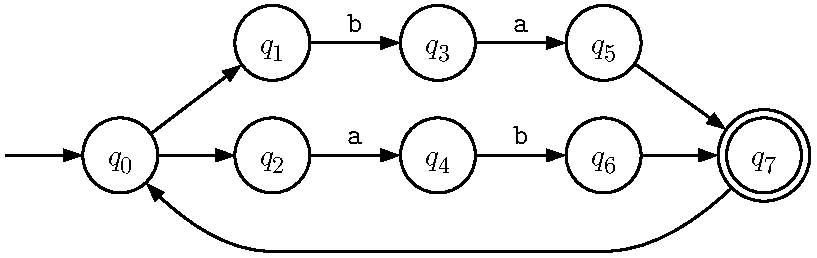
\includegraphics[scale=0.8]{Abbildungen/ab-or-ba-star.pdf}

   \caption{An \simtextsc{Nfa} with $\varepsilon$-transitions.}
  \label{fig:ab-or-ba-star.dot}
\end{figure}

\exampleEng
Figure \ref{fig:ab-or-ba-star.dot} shows an \simtextsc{Nfa} with 
$\varepsilon$-transitions.   In this figure, the $\varepsilon$-transitions are shown as unlabelled arrows.
We compute the $\varepsilon$-closure for all states:
\begin{enumerate}
\item $\textsl{ec}(q_0) = \{ q_0, q_1, q_2 \}$,
\item $\textsl{ec}(q_1) = \{ q_1 \}$,
\item $\textsl{ec}(q_2) = \{ q_2 \}$,
\item $\textsl{ec}(q_3) = \{ q_3 \}$,
\item $\textsl{ec}(q_4) = \{ q_4 \}$,
\item $\textsl{ec}(q_5) = \{ q_5, q_7, q_0, q_1, q_2 \}$,
\item $\textsl{ec}(q_6) = \{ q_6, q_7, q_0, q_1, q_2 \}$,
\item $\textsl{ec}(q_7) = \{ q_7, q_0, q_1, q_2 \}$.
\end{enumerate}
For example, the fixpoint iteration that computes $\textsl{ec}(q_5)$ yields the sets
\\[0.2cm]
\hspace*{1.3cm}
$M_0 = \{ q_5 \}$, \quad $M_1 = \{ q_5, q_7 \}$, \quad $M_2 = \{ q_5, q_7, q_0 \}$,
\\[0.2cm]
\hspace*{1.3cm}
$M_3 = \{ q_5, q_7, q_0, q_1, q_2 \}$, \quad and \quad $M_4 = M_3$.
\qed

\noindent
In order to transform an \simtextsc{Nfa} into a  \simtextsc{Dfa}
$\textsl{det}(F)$ we have to extend the function $\delta:Q  \times (\Sigma \cup \{\varepsilon\}) \rightarrow 2^Q$ into the function
\\[0.2cm]
\hspace*{1.3cm}
$\widehat{\delta}: Q \times \Sigma \rightarrow 2^Q$.
\\[0.2cm]
The idea is that given a state $q$ and a character $c$,  $\widehat{\delta}(q,c)$ is the set of all states that 
$F$ could reach when it reads the character $c$ in state $q$ and then performs an arbitrary number
of $\varepsilon$-transitions.  Formally, the definition of $\widehat{\delta}$ is as follows:
\\[0.2cm]
\hspace*{1.3cm}
$\ds \widehat{\delta}(q_1, c) := \bigcup \bigl\{ \textsl{ec}(q_2) \bigm| q_2 \in \delta(q_1, c) \bigr \}$.
\\[0.2cm]
This formula is to be read as follows:
\begin{enumerate}[(a)]
\item For every state $q_2 \in Q$ that can be reached from the state $q_1$ by reading the character $c$ we
      compute the $\varepsilon$-closure $\textsl{ec}(q_2)$.
\item Then we take the union of all the sets $\textsl{ec}(q_2)$ where $q_2 \in \delta(q_1, c)$.
\end{enumerate}

\exampleEng
In continuation of the previous example (shown in Figure \ref{fig:ab-or-ba-star.dot}) we have:
\begin{enumerate}
\item $\widehat{\delta}(q_0, \texttt{a}) = \{\}$,
  
      because in state $q_0$ there is no transition on reading the character \texttt{a}.
      Note that in our definition of the function  $\widehat{\delta}$ the 
      $\varepsilon$-transitions are done only after the character has been read.
\item $\widehat{\delta}(q_1, \texttt{b}) = \{q_3\}$,

      because when the letter \texttt{'b'} is read in the state $q_1$ the \simtextsc{Nfa}
      switches into the state $q_3$ and the state $q_3$ has no  $\varepsilon$-transitions.
\item $\widehat{\delta}(q_3, \texttt{a}) = \{q_5, q_7, q_0, q_1, q_2\}$,

      because when the letter \texttt{'a'} is read in the state $q_3$ the \simtextsc{Nfa}
      switches into the state $q_5$.  From $q_5$ the states $q_7$, $q_0$, $q_1$ and $q_2$
      are reachable by $\varepsilon$-transitions. \eox
\end{enumerate}
The function  $\widehat{\delta}$ takes a state and a character and maps it into a set of states.  Since  $\textsl{det}(F)$ uses
sets of states of $F$ as its states we need a function that takes a set of states and a character and maps it
into a set of states.
Hence we generalize the function $\widehat{\delta}$ to the function
\\[0.2cm]
\hspace*{1.3cm}
$\Delta: 2^Q \times \Sigma \rightarrow 2^Q$
\\[0.2cm]
such that for a set $M$ of states and a character $c$ the expression $\Delta(M, c)$
computes the set of all those states that $F$ could be in if it is in a state from $M$, then
reads the character $c$, and finally makes some $\varepsilon$-transitions.
The formal definition is as follows: 
\\[0.2cm]
\hspace*{1.3cm}
$\ds \Delta(M,c) := \bigcup \Bigl\{ \widehat{\delta}(q,c) \bigm| q \in M \Bigr\}$. 
\\[0.2cm]
This formula is easy to understand:  For every state  $q \in M$ we compute the set of states that 
$F$ could be in after reading the character $c$ and doing some 
$\varepsilon$-transitions afterwards.  Then we take the union of these sets.

\exampleEng
Continuing our previous example (shown in Figure \ref{fig:ab-or-ba-star.dot}) we have:
\begin{enumerate}
\item $\Delta(\{q_0, q_1, q_2\}, \texttt{a}) = \{ q_4 \}$,
\item $\Delta(\{q_0, q_1, q_2\}, \texttt{b}) = \{ q_3 \}$,
\item $\Delta(\{ q_3 \}, \texttt{a}) = \{ q_5, q_7, q_0, q_1, q_2 \}$,
\item $\Delta(\{ q_3 \}, \texttt{b}) = \{ \}$,
\item $\Delta(\{ q_4 \}, \texttt{a}) = \{ \}$,
\item $\Delta(\{ q_4 \}, \texttt{b}) = \{ q_6, q_7, q_0, q_1, q_2 \}$.
      \eox
\end{enumerate}
Now we are ready to formally define how $\textsl{det}(F)$ is constructed from $F := \bigl\langle Q, \Sigma, \delta, q_0, A \bigr\rangle$.
\\[0.2cm]
\hspace*{1.3cm}
$\textsl{det}(F) := \bigl\langle 2^Q, \Sigma, \Delta, \textsl{ec}(q_0), \widehat{A} \bigr\rangle$
\index{$\textsl{det}(F)$}\glsadd{det} 
\\[0.2cm]
where the components of this tuple are defined as follows:
\begin{enumerate}
\item The set of states of $\textsl{det}(F)$ is the set of all subsets of $Q$ and therefore it is equal to the power set
      $2^Q$.

      Later we will see that we do not need all of these subsets.
      The reason is that the states are those subsets that can be reached from the start state $q_0$ 
      when some string has been read.  In most cases there are some combinations of states that cannot be reached
      and the corresponding sets are not really needed as states.
\item The input alphabet $\Sigma$ does not change when going from $F$ to $\textsl{det}(F)$.
      After all, the finite state machine $\textsl{det}(F)$ has to recognize the same language as $F$.
\item The previously defined function $\Delta$ specifies how the set of states changes when a
      character is read.
\item The start state $\textsl{ec}(q_0)$ of $\textsl{det}(F)$ is the set of all states
      that can be reached from the start state $q_0$ of $F$ via $\varepsilon$-transitions.
\item The set of accepting states $\widehat{A}$ is the set of those subsets of $Q$ that do contain an accepting
      state of $F$:
      \\[0.2cm]
      \hspace*{1.3cm}
      $\widehat{A} := \bigl\{ M \in 2^Q \mid M \cap A \not= \{\} \bigr\}$.
\end{enumerate}

\exerciseEng
Transform the \simtextsc{Nfa} $F$ that is shown in Figure \ref{fig:abstarbabab-nd.dot} on page
\pageref{fig:abstarbabab-nd.dot}  into a \simtextsc{Dfa} $\textsl{det}(F)$.  \eox

\solutionEng
We start by computing the set of states.
\begin{enumerate}
\item As we have $\textsl{ec}(0) = \{0\}$, the start state of $\textsl{det}(F)$  is the set containing $0$.
      \\[0.2cm]
      \hspace*{1.3cm}
      $S_0 := \textsl{ec}(0) = \{ 0 \}$.
\item As we have $\delta(0, \texttt{a}) = \{0\}$ and there are no $\varepsilon$-transitions we have
      \\[0.2cm]
      \hspace*{1.3cm}
      $\Delta(S_0, \texttt{a}) = \Delta(\{0\}, \texttt{a}) = \{0\} = S_0$.
\item As we have $\delta(0, \texttt{b}) = \{0, 1\}$ we conclude
      \\[0.2cm]
      \hspace*{1.3cm}
      $S_1 := \Delta(S_0, \texttt{b}) = \Delta(\{0\}, \texttt{b}) = \{ 0, 1 \}$.
\item We have that $\delta(0, \texttt{a}) = \{ 0 \}$ and $\delta(1, \texttt{a}) = \{ 2 \}$.
      Hence
      \\[0.2cm]
      \hspace*{1.3cm}
      $S_2 := \Delta(S_1, \texttt{a}) = \Delta(\{ 0, 1 \}, \texttt{a}) = \{ 0, 2 \}$.
\item We have $\delta(0, \texttt{b}) = \{ 0, 1 \}$ and $\delta(1, \texttt{b}) = \{ 2 \}$.
      Therefore
      \\[0.2cm]
      \hspace*{1.3cm}
      $S_3 := \Delta(S_1, \texttt{b}) = \Delta(\{ 0, 1 \}, \texttt{b}) = \{ 0, 1, 2 \}$

      Similarly we derive the following:
\item $S_4 := \Delta(S_2, \texttt{a}) = \Delta(\{ 0, 2 \}, \texttt{a}) = \{0, 3 \}$.
\item $S_5 := \Delta(S_2, \texttt{b}) = \Delta(\{ 0, 2 \}, \texttt{b}) = \{0, 1, 3 \}$.
\item $S_6 := \Delta(S_3, \texttt{a}) = \Delta(\{ 0, 1, 2 \}, \texttt{a}) = \{0, 2, 3 \}$.
\item $S_7 := \Delta(S_3, \texttt{b}) = \Delta(\{ 0, 1, 2 \}, \texttt{b}) = \{0, 1, 2, 3 \}$.
\item $\Delta(S_4, \texttt{a}) = \Delta(\{ 0, 3 \}, \texttt{a}) = \{0 \} = S_0$.
\item $\Delta(S_4, \texttt{b}) = \Delta(\{ 0, 3 \}, \texttt{b}) = \{ 0, 1 \} = S_1$.
\item $\Delta(S_5, \texttt{a}) = \Delta(\{ 0, 1, 3 \}, \texttt{a}) = \{ 0, 2 \} = S_2$.
\item $\Delta(S_5, \texttt{b}) = \Delta(\{ 0, 1, 3 \}, \texttt{b}) = \{ 0, 1, 2 \} = S_3$.
\item $\Delta(S_6, \texttt{a}) = \Delta(\{ 0, 2, 3 \}, \texttt{a}) = \{ 0, 3 \} = S_4$.
\item $\Delta(S_6, \texttt{b}) = \Delta(\{ 0, 2, 3 \}, \texttt{b}) = \{ 0, 1, 3 \} = S_5$.
\item $\Delta(S_7, \texttt{a}) = \Delta(\{ 0, 1, 2, 3 \}, \texttt{a}) = \{ 0, 2, 3 \} = S_6$.
\item $\Delta(S_7, \texttt{b}) = \Delta(\{ 0, 1, 2, 3 \}, \texttt{b}) = \{ 0, 1, 2, 3 \} = S_7$.
\end{enumerate}
These are all possible sets of states that the \simtextsc{Dfa} $\textsl{det}(F)$ can reach.
For a better overview let us summarize the definitions of the individual states of the \simtextsc{Dfa} $\textsl{det}(F)$:
\\[0.2cm]
\hspace*{1.3cm} $S_0 = \{ 0 \}$, $S_1 = \{ 0, 1 \}$, $S_2 = \{ 0, 2 \}$,  $S_3 = \{ 0, 1, 2 \}$, $S_4 = \{ 0, 3 \}$,
\\[0.2cm]
\hspace*{1.3cm} $S_5 = \{ 0, 1, 3 \}$, $S_6 = \{ 0, 2, 3 \}$, $S_7 = \{ 0, 1, 2, 3 \}$
\\[0.2cm]
Therefore the set $\widehat{Q}$ of the states of $\textsl{det}(F)$ is given as follows:
\\[0.2cm]
\hspace*{1.3cm}
$\widehat{Q} := \{ S_0, S_1, S_2, S_3, S_4, S_5, S_6, S_7 \}$.
\\[0.2cm]
The transition function $\Delta$ is shown as a table:

\begin{center}
\begin{tabular}[t]{|l||c|c|c|c|c|c|c|c|}
\hline
$\Delta$ & $S_0$ & $S_1$ & $S_2$ & $S_3$ & $S_4$ & $S_5$ & $S_6$ & $S_7$ \\
\hline
\hline
\texttt{a} & $S_0$ & $S_2$ & $S_4$ & $S_6$ & $S_0$ & $S_2$ & $S_4$ & $S_6$ \\
\hline
\texttt{b} & $S_1$ & $S_3$ & $S_5$ & $S_7$ & $S_1$ & $S_3$ & $S_5$ & $S_7$ \\
\hline
\end{tabular}
\end{center}
Finally we recognize that only the sets  $S_4$, $S_5$, $S_6$ and $S_7$ contain the accepting state
 $3$.  Therefore we have
\\[0.2cm]
\hspace*{1.3cm}
$\widehat{A} := \{ S_4, S_5, S_6, S_7 \}$.
\\[0.2cm]
Therefore we have now found $\textsl{det}(F)$. We have
\\[0.2cm]
\hspace*{1.3cm}
$\textsl{det}(F) := \langle \widehat{Q}, \Sigma, \Delta, S_0, \widehat{A}\rangle$.
\\[0.2cm]
This \simtextsc{Dfa} is shown in Figure \ref{fig:a2.eps} on page \pageref{fig:a2.eps}.

We realize that $\textsl{det}(F)$ has 8 different states. 
The \simtextsc{Nfa} $F$ has 4 different states
 $Q = \{ 0, 1, 2, 3 \}$.  Hence the power set $2^Q$ has 16 elements.
Why then has  $\textsl{det}(F)$ only 8 and not $2^4 = 16$ states?
The reason is that we can only reach those sets of states from the start $0$
that contain the state $0$ because no matter whether we read an \texttt{a} or a \texttt{b},
 $F$ can always choose to switch to the state $0$.  Therefore, every set of states that is
reachable from the state $0$ has to contain the state $0$.  Therefore,
sets that do not contain $0$ are not needed as states of $\textsl{det}(F)$.

The computation of the states $S_0$, $\cdots$, $S_7$ in the solution above is another fixpoint iteration.  The set
of those states of $\textsl{det}(F)$ that can be reached from the start state $\textsl{ec}(q_0)$ is the smallest set
$\mathcal{S}$ such that $\textsl{ec}(q_0) \in \mathcal{S}$ holds and such that $\mathcal{S}$ is a fixpoint of the
function
\\[0.2cm]
\hspace*{1.3cm}
$\textsl{allStatesStep}(\mathcal{S}) := \mathcal{S} \cup \bigl\{ \Delta(M, c) \bigm| M \in \mathcal{S} \wedge c \in \Sigma \bigr\}$.
\\[0.2cm]
The equation $\textsl{allStatesStep}(\mathcal{S}) = \mathcal{S}$ states that every state that can be reached from a
state in $\mathcal{S}$ by reading a single character is already an element of $\mathcal{S}$.  The fixpoint iteration
starts with the set $\mathcal{S}_0 := \bigl\{ \textsl{ec}(q_0) \bigr\}$.  Then the set $\mathcal{S}_n$ contains
exactly those states of $\textsl{det}(F)$ that can be reached from the start state by reading at most $n$
characters.  As all these sets are subsets of the finite set $2^Q$, the iteration terminates.  For the
\simtextsc{Nfa} of the exercise, it computes the sets
\\[0.2cm]
\hspace*{1.3cm}
$\mathcal{S}_0 = \{ S_0 \}$, \quad $\mathcal{S}_1 = \{ S_0, S_1 \}$, \quad
$\mathcal{S}_2 = \{ S_0, S_1, S_2, S_3 \}$, \quad $\mathcal{S}_3 = \{ S_0, S_1, \cdots, S_7 \}$, \quad and \quad
$\mathcal{S}_4 = \mathcal{S}_3$.



\begin{figure}[!ht]
  \centering
     \vspace*{0.5cm}
      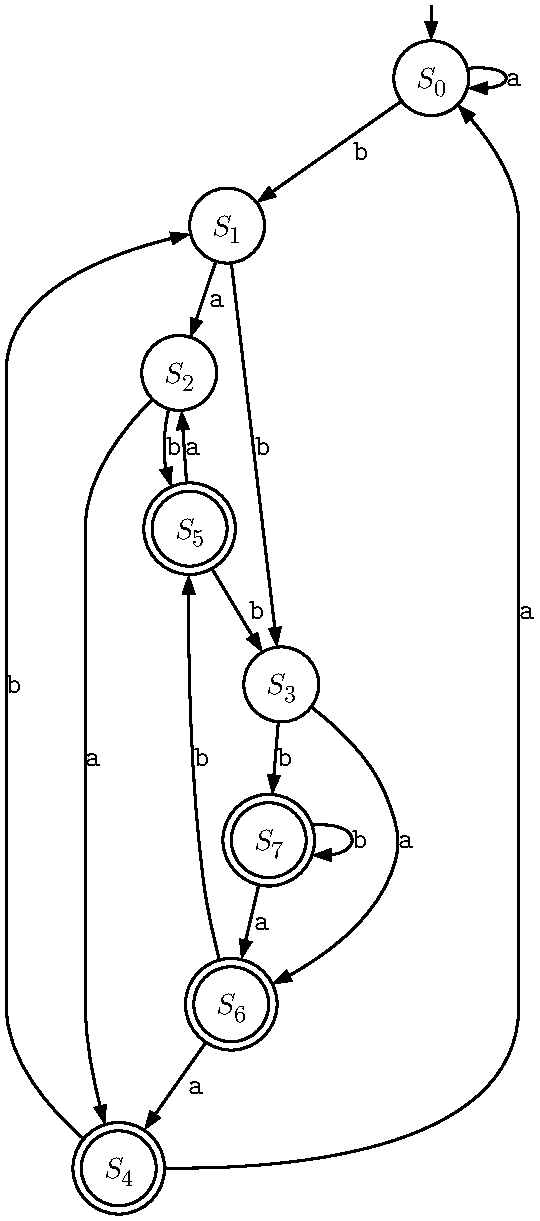
\includegraphics[scale=0.8]{Abbildungen/a2.pdf}
  \caption{The \simtextsc{Dfa} $\textsl{det}(F)$.}
  \label{fig:a2.eps}
\end{figure}


\exerciseEng
Transform the \simtextsc{Nfa} $F$ that is shown in Figure \ref{fig:ab-or-ba-star.dot} on page
\pageref{fig:ab-or-ba-star.dot} 
into an equivalent \simtextsc{Dfa} $\textsl{det}(F)$. \eox

\subsection{Implementation}
It is straightforward to implement the theory developed so far.
The \textsl{Jupyter notebook}
\\[0.2cm]
\hspace*{1.3cm}
\href{https://github.com/karlstroetmann/Formal-Languages/blob/master/Python/Chapter-04-05/01-NFA-2-DFA.ipynb}{\texttt{Python/Chapter-04-05/01-NFA-2-DFA.ipynb}}
\\[0.2cm]
contains a program that takes a \simtextsc{Nfa} $F$ and computes the \simtextsc{Dfa} $\textsl{det}(F)$.  In this
subsection and in the implementation subsections of the following sections, we discuss the notebooks of this
chapter line by line.  To keep the listings short, they show a simplified version of the code in the notebooks:  We
have removed the type annotations, and a few long lines have been split into two lines.

\begin{figure}[!ht]
\centering
\begin{minted}[ frame         = lines,
                framesep      = 0.3cm,
                firstnumber   = 1,
                bgcolor       = sepia,
                numbers       = left,
                numbersep     = 0.3cm,
                xleftmargin   = 0.5cm,
                xrightmargin  = 0.5cm,
                gobble        = 4,
              ]{python3}
    State = TypeVar('State')
    Char = str
    Delta = dict[tuple[State, Char], set[State]]
    TransRel = dict[tuple[State, Char], State]
    NFA = tuple[set[State], set[Char], Delta, State, set[State]]
    DFA = tuple[set[State], set[Char], TransRel, State, set[State]]
\end{minted}
\vspace*{-0.3cm}
\caption{The types that represent finite state machines.}
\label{fig:01-NFA-2-DFA.ipynb:types}
\end{figure}

\noindent
Figure \ref{fig:01-NFA-2-DFA.ipynb:types} on page \pageref{fig:01-NFA-2-DFA.ipynb:types} shows how the notebook
represents finite state machines.  The other notebooks of this chapter use the same representation.
\begin{enumerate}
\item Line 1 defines the \blue{type variable}\index{type variable} \texttt{State}.  It stands for the type of the
      states, which is left open, since the functions of the notebook work for states of any type.  For example,
      the states of the \simtextsc{Nfa}s that are constructed in the next section are numbers, while the states of
      $\textsl{det}(F)$ are sets of states of $F$.
\item Line 2 defines the type \texttt{Char} of characters.  As \textsl{Python} has no type of its own for
      characters, a character is represented as a string of length one.
\item Line 3 defines the type \texttt{Delta} of the transition function
      $\delta: Q \times (\Sigma \cup \{\varepsilon\}) \rightarrow 2^Q$ of a \simtextsc{Nfa}.  This function is
      stored as a dictionary that maps a pair $\pair(q, c)$ to the set $\delta(q, c)$.  The character
      $\varepsilon$ is represented by the string \texttt{'𝜀'}.  If $\delta(q, c)$ is the empty set, the
      dictionary need not contain the pair $\pair(q, c)$ as a key.
\item Line 4 defines the type \texttt{TransRel} of the transition function
      $\delta: Q \times \Sigma \rightarrow Q \cup \{\Omega\}$ of a \simtextsc{Dfa}.  This dictionary maps a pair
      $\pair(q, c)$ to the state $\delta(q, c)$.  If $\delta(q, c) = \Omega$, the dictionary does not contain the
      pair $\pair(q, c)$ as a key.
\item Line 5 -- 6 define the types \texttt{NFA} and \texttt{DFA}.  A finite state machine
      $\langle Q, \Sigma, \delta, q_0, A \rangle$ is represented as a tuple with five components, where the set of
      states $Q$, the alphabet $\Sigma$, and the set of accepting states $A$ are \textsl{Python} sets.
\end{enumerate}
The states of the \simtextsc{Dfa} that the notebook computes are only those subsets of $Q$ that can be reached
from the start state $\textsl{ec}(q_0)$.  As both the $\varepsilon$-closure and the set of these states are
computed by a fixpoint iteration, the notebook implements the fixpoint iteration as a function of its own.  Figure
\ref{fig:01-NFA-2-DFA.ipynb:fixpoint} on page \pageref{fig:01-NFA-2-DFA.ipynb:fixpoint} shows this function
together with the functions that use it.

\begin{figure}[!ht]
\centering
\begin{minted}[ frame         = lines,
                framesep      = 0.3cm,
                firstnumber   = 1,
                bgcolor       = sepia,
                numbers       = left,
                numbersep     = 0.3cm,
                xleftmargin   = 0.5cm,
                xrightmargin  = 0.5cm,
                gobble        = 4,
              ]{python3}
    def fixpoint(f, x, *args):
        while True:
            y = f(x, *args)
            if y == x:
                return x
            x = y

    def epsClosureStep(M, δ):
        return M | bigUnion({ frozenset(δ.get((q, '𝜀'), set()))
                              for q in M })

    def epsClosure(s, δ):
        return fixpoint(epsClosureStep, frozenset({ s }), δ)

    def allStatesStep(S, δ, Σ):
        return S | { capitalDelta(M, c, δ) for M in S
                                           for c in Σ
                   }

    def allStates(Q, δ, Σ):
        return fixpoint(allStatesStep, { Q }, δ, Σ)
\end{minted}
\vspace*{-0.3cm}
\caption{The function \texttt{fixpoint} and the functions that compute the $\varepsilon$-closure and the states of
  $\textsl{det}(F)$.}
\label{fig:01-NFA-2-DFA.ipynb:fixpoint}
\end{figure}

\begin{enumerate}
\item Line 1 -- 6 define the function \texttt{fixpoint}.  Given a function \texttt{f}, a start value \texttt{x},
      and additional arguments \texttt{args}, it computes the values
      \\[0.2cm]
      \hspace*{1.3cm}
      \texttt{x}, \quad \texttt{f(x, *args)}, \quad \texttt{f(f(x, *args), *args)}, \quad $\cdots$
      \\[0.2cm]
      until it finds a fixpoint, i.e.~a value \texttt{y} that does not change when \texttt{f} is applied to it,
      and returns this value.  The additional arguments are passed to \texttt{f} in every call.  They are needed, since the functions
      $\textsl{ecStep}$ and $\textsl{allStatesStep}$ depend on the transition function $\delta$ and the function
      $\textsl{allStatesStep}$ also depends on the alphabet $\Sigma$.
\item Line 8 -- 10 define the function \texttt{epsClosureStep}, which implements the function $\textsl{ecStep}$.
      As the dictionary $\delta$ need not have an entry for a state without $\varepsilon$-transitions, the
      expression
      \\[0.2cm]
      \hspace*{1.3cm}
      \texttt{δ.get((q, '𝜀'), set())}
      \\[0.2cm]
      returns the empty set in this case.  The function \texttt{bigUnion}, which is shown in Figure
      \ref{fig:01-NFA-2-DFA.ipynb:nfa2dfa} on page \pageref{fig:01-NFA-2-DFA.ipynb:nfa2dfa}, computes the union
      $\bigcup$ of a set of sets.  As it expects a set of \texttt{frozenset}s, the sets $\delta(q, \varepsilon)$
      are converted into \texttt{frozenset}s.
\item Line 12 -- 13 define the function \texttt{epsClosure}, which computes $\textsl{ec}(s)$ by a fixpoint
      iteration that starts with the set $\{ s \}$.
\item Line 15 -- 18 define the function \texttt{allStatesStep}, which implements the function
      $\textsl{allStatesStep}$.  The function \texttt{capitalDelta}, which is also shown in Figure
      \ref{fig:01-NFA-2-DFA.ipynb:nfa2dfa}, implements the function $\Delta$.
\item Line 20 -- 21 define the function \texttt{allStates}.  Its argument \texttt{Q} is the start state
      $\textsl{ec}(q_0)$ of $\textsl{det}(F)$.  The function computes the set of all states of
      $\textsl{det}(F)$ that can be reached from \texttt{Q} by a fixpoint iteration that starts with the set
      $\{ \texttt{Q} \}$.
\end{enumerate}

\begin{figure}[!ht]
\centering
\begin{minted}[ frame         = lines,
                framesep      = 0.3cm,
                firstnumber   = 1,
                bgcolor       = sepia,
                numbers       = left,
                numbersep     = 0.3cm,
                xleftmargin   = 0.5cm,
                xrightmargin  = 0.5cm,
                gobble        = 4,
              ]{python3}
    def bigUnion(M):
        return frozenset({ x for A in M
                             for x in A
                         })

    def deltaHat(s, c, δ):
        return bigUnion({ epsClosure(q, δ)
                          for q in δ.get((s, c), set()) })

    def capitalDelta(M, c, δ):
        return bigUnion({ deltaHat(q, c, δ) for q in M })

    def nfa2dfa(nfa):
        _, Σ, δ, q0, Final = nfa
        newStart  = epsClosure(q0, δ)
        NewStates = allStates(newStart, δ, Σ)
        newδ  = { (M, c): capitalDelta(M, c, δ) for M in NewStates
                                                for c in Σ
                }
        NewFinal = { M for M in NewStates if  M & Final != set() }
        return NewStates, Σ, newδ, newStart, NewFinal
\end{minted}
\vspace*{-0.3cm}
\caption{The functions \texttt{bigUnion}, \texttt{deltaHat}, \texttt{capitalDelta}, and \texttt{nfa2dfa}.}
\label{fig:01-NFA-2-DFA.ipynb:nfa2dfa}
\end{figure}

\noindent
Figure \ref{fig:01-NFA-2-DFA.ipynb:nfa2dfa} on page \pageref{fig:01-NFA-2-DFA.ipynb:nfa2dfa} shows the remaining
functions of the notebook.
\begin{enumerate}
\item Line 1 -- 4 define the function \texttt{bigUnion}.  Given a set $M$ of sets, it computes the union
      \\[0.2cm]
      \hspace*{1.3cm}
      $\ds \bigcup M = \bigl\{ x \bigm| \exists A \in M: x \in A \bigr\}$
      \\[0.2cm]
      with a set comprehension that iterates over all sets $A$ in $M$ and all elements $x$ of $A$.  The result
      is returned as a \texttt{frozenset}.  The reason is that \textsl{Python} finds the elements of a set and
      the keys of a dictionary via their hash values.  Therefore, these elements and keys must not change.  As a
      set can be changed, it can neither be an element of a set nor a key of a dictionary.  In contrast, a
      \texttt{frozenset} cannot be changed after it has been created.  As the states of $\textsl{det}(F)$ are
      sets of states of $F$, which are elements of the set of states of $\textsl{det}(F)$ and occur in the keys
      of its transition function, they are represented as \texttt{frozenset}s.  For the same reason, the
      argument $M$ of \texttt{bigUnion} is a set of \texttt{frozenset}s.
\item Line 6 -- 8 define the function \texttt{deltaHat}, which implements the function $\widehat{\delta}$:
      \\[0.2cm]
      \hspace*{1.3cm}
      $\ds\widehat{\delta}(q_1, c) = \bigcup \bigl\{ \textsl{ec}(q_2) \bigm| q_2 \in \delta(q_1, c) \bigr\}$.
      \\[0.2cm]
      As in the function \texttt{epsClosureStep}, the method \texttt{get} returns the empty set if there is no
      transition from the state \texttt{s} for the character \texttt{c}.
\item Line 10 -- 11 define the function \texttt{capitalDelta}, which implements the function $\Delta$:
      \\[0.2cm]
      \hspace*{1.3cm}
      $\ds\Delta(M,c) = \bigcup \bigl\{ \widehat{\delta}(q,c) \bigm| q \in M \bigr\}$.
\item Line 13 -- 21 define the function \texttt{nfa2dfa}, which computes $\textsl{det}(F)$ for the
      \simtextsc{Nfa} $F$ that is given as the argument \texttt{nfa}.
      \begin{enumerate}
      \item Line 14 extracts the components of $F$.  The set of states of $F$ is not needed.  Therefore, it is
            assigned to the variable \texttt{\_}, which, by convention, holds values that are not used.
      \item Line 15 computes the start state $\textsl{ec}(q_0)$ of $\textsl{det}(F)$.
      \item Line 16 computes the set of states of $\textsl{det}(F)$.  Instead of the power set $2^Q$, which
            occurs in the definition of $\textsl{det}(F)$, it contains only those sets of states that can be
            reached from the start state.
      \item Line 17 -- 19 compute the transition function $\Delta$ of $\textsl{det}(F)$ as a dictionary.  As the
            set \texttt{NewStates} is a fixpoint of the function \texttt{allStatesStep}, the set
            $\Delta(M, c)$ is an element of \texttt{NewStates} for every $M \in \texttt{NewStates}$ and every
            $c \in \Sigma$.  Hence $\textsl{det}(F)$ is complete:  If $F$ dies in all states of $M$ when it
            reads the character $c$, then $\Delta(M, c)$ is the empty set.  In this case, the empty set is a state
            of $\textsl{det}(F)$.  It is not accepting and all of its transitions lead back to it.
      \item Line 20 computes the set $\widehat{A}$ of accepting states.  The operator ``\texttt{\&}'' computes
            the intersection of two sets.
      \item Line 21 returns the five components of $\textsl{det}(F)$.
      \end{enumerate}
\end{enumerate}
The notebook
\href{https://github.com/karlstroetmann/Formal-Languages/blob/master/Python/Chapter-04-05/02-Test-NFA-2-DFA.ipynb}{\texttt{02-Test-NFA-2-DFA.ipynb}}
applies the function \texttt{nfa2dfa} to the \simtextsc{Nfa} shown in Figure \ref{fig:ab-or-ba-star.dot} on page
\pageref{fig:ab-or-ba-star.dot}.  It draws both finite state machines with the help of the notebook
\href{https://github.com/karlstroetmann/Formal-Languages/blob/master/Python/Chapter-04-05/FSM-2-Dot.ipynb}{\texttt{FSM-2-Dot.ipynb}},
which uses the program \textsl{Graphviz}.


\section{From Regular Expression to NFAs \label{section:regexp-2-nfa}}
In this section we show how a regular expression can be implemented as an \simtextsc{Nfa}.
Given a regular expression $r$ we will construct an \simtextsc{Nfa} $A(r)$ that accepts the
language that is described by the regular expression $r$, i.e.~we will have
\\[0.2cm]
\hspace*{1.3cm}
$L\bigl(A(r)\bigr) = L(r)$.
\\[0.2cm]
The \simtextsc{Nfa} $A(r)$ is defined by induction on the regular expression $r$.  The \simtextsc{Nfa} $A(r)$ will
have the following properties:
\begin{enumerate}
\item $A(r)$ does not have a transition into its start state.  
\item $A(r)$ has exactly one accepting state.  
      Furthermore, there are no transitions out of this state.
\end{enumerate}
In the following we assume that $\Sigma$ is the alphabet that has been used when constructing the regular
expression $r$.  Then we can define $A(r)$ as follows:
\begin{enumerate}
\item The \simtextsc{Nfa} $A(\emptyset)$ is defined as
      \\[0.2cm]
      \hspace*{1.3cm}
      $A(\emptyset) = \bigl\langle \{ q_0, q_1 \}, \Sigma, \{\}, q_0, \{ q_1 \} \bigr\rangle$.
      \\[0.2cm]
      Note that this \simtextsc{Nfa} has no transitions at all.

      \begin{figure}[!ht]
        \centering
      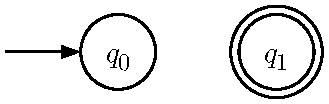
\includegraphics[scale=0.8]{Abbildungen/aLeer.pdf}
      \caption{The \simtextsc{Nfa} $A(\emptyset)$.}
      \label{fig:aLeer.eps}
      \end{figure}
      Figure \ref{fig:aLeer.eps} shows the \simtextsc{Nfa} $A(\emptyset)$. It is obvious that we have
      $L\bigl(A(\emptyset)\bigr) = \{\}$. 
\item The \simtextsc{Nfa} $A(\varepsilon)$ is defined as
      \\[0.2cm]
      \hspace*{1.3cm}
      $A(\varepsilon) = \bigl\langle \{ q_0, q_1 \}, \Sigma, 
                          \bigl\{ \pair(q_0, \varepsilon) \mapsto \{q_1\} \bigr\}, q_0, \{ q_1 \} \bigr\rangle$.


      \begin{figure}[!ht]
        \centering
      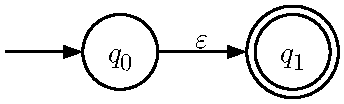
\includegraphics[scale=0.8]{Abbildungen/aEpsilon.pdf}
      \caption{The \simtextsc{Nfa} $A(\varepsilon)$.}
      \label{fig:aEpsilon.eps}
      \end{figure}
      Figure \ref{fig:aEpsilon.eps} shows the \simtextsc{Nfa} $A(\varepsilon)$.
      We have that $L\bigl(A(\varepsilon)\bigr) = \{\lambda\}$, i.e.~the \simtextsc{Nfa} accepts only the empty string. 
\item For a letter $c \in \Sigma$ the \simtextsc{Nfa} $A(c)$ is defined as 
      \\[0.2cm]
      \hspace*{1.3cm}
      $A(c) = \bigl\langle \{ q_0, q_1 \}, \Sigma, 
                                \bigl\{ \langle q_0, c \rangle \mapsto \{q_1\}\bigr\}, q_0, \{ q_1 \} \bigr\rangle$.

      \begin{figure}[!ht]
        \centering
      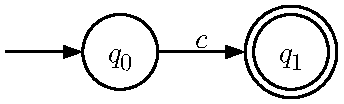
\includegraphics[scale=0.8]{Abbildungen/aChar.pdf}
      \caption{The \simtextsc{Nfa} $A(c)$.}
      \label{fig:aChar.eps}
      \end{figure}
      Figure \ref{fig:aChar.eps} shows $A(c)$.
      We have that $L\bigl(A(c)\bigr) = \{c\}$, i.e.~the \simtextsc{Nfa} accepts only the character $c$. 
\item In order to define the \simtextsc{Nfa} $A(r_1 \cdot r_2)$ for the concatenation $r_1 \cdot r_2$ 
      we assume that we have already constructed \simtextsc{Nfa}s $A(r_1)$ and $A(r_2)$
      such that $L\bigl(A(r_1)\bigr) = L(r_1)$ and $L\bigl(A(r_2)\bigr) = L(r_2)$.  Furthermore,
      without loss of generality we assume that the states in the \simtextsc{Nfa}s  $A(r_1)$ and $A(r_2)$ are different. 
      This can always be achieved by renaming the states of $A(r_2)$.
      Next, we assume that $A(r_1)$ and $A(r_2)$ have the following form:
      \begin{enumerate}
      \item $A(r_1) = \bigl\langle Q_1, \Sigma, \delta_1, q_1, \{ q_2 \}\bigr\rangle$,
      \item $A(r_2) = \bigl\langle Q_2, \Sigma, \delta_2, q_3, \{ q_4 \}\bigr\rangle$,
      \item $Q_1 \cap Q_2 = \{\}$.
      \end{enumerate}
      Then we can build the \simtextsc{Nfa} $A(r_1 \cdot r_2)$ from $A(r_1)$ and $A(r_2)$ as follows:
      \\[0.2cm]
      \hspace*{0.8cm}
       $A(r_1 \cdot r_2) := \bigl\langle Q_1 \cup Q_2, \Sigma, 
                \bigl\{ \pair(q_2,\varepsilon) \mapsto \{q_3\} \bigr\} 
                   \cup \delta_1 \cup \delta_2, q_1, \{ q_4 \} \bigr\rangle$
      \\[0.2cm]
      Here, the notation $\{ \pair(q_2,\varepsilon) \mapsto \{q_3\} \} \cup \delta_1 \cup \delta_2$ specifies that
      $A(r_1 \cdot r_2)$ contains all transitions from both $A(r_1)$ and $A(r_2)$ and, furthermore,
      contains an $\varepsilon$-transition from $q_2$ to $q_3$.     
      Formally, this transition function  $\delta$ can be specified as follows:
      \\[0.2cm]
      \hspace*{1.3cm}
      $\delta(q,c) := \left\{
      \begin{array}{ll}
        \{ q_3 \}       & \mbox{if $q = q_2$ and $c = \varepsilon$}, \\[0.2cm]
        \delta_1(q, c)  & \mbox{if $q \in Q_1$ and $\pair(q,c) \not= \pair(q_2,\varepsilon)$}, \\[0.2cm]
        \delta_2(q, c)  & \mbox{if $q \in Q_2$.} 
      \end{array}\right.
      $
      \\[0.2cm]


      \begin{figure}[!ht]
        \centering
      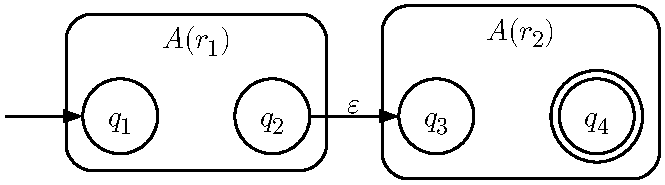
\includegraphics[scale=0.8]{Abbildungen/aConcat.pdf}
      \caption{The \simtextsc{Nfa} $A(r_1 \cdot r_2)$.}
      \label{fig:aConcat.eps}
      \end{figure}
      Figure \ref{fig:aConcat.eps} shows the \simtextsc{Nfa} $A(r_1 \cdot r_2)$.

      Instead of having an $\varepsilon$-transition from $q_2$ to $q_3$ we can identify the states $q_2$ and
      $q_3$.  The advantage is that the resulting \simtextsc{Nfa} is smaller.
      We will do this when creating \simtextsc{Nfa}s by hand.  

      I haven't done this identification in the definition above because both the graphical representation and 
      the implementation get more complicated if we identify these states.
\item In order to define the \simtextsc{Nfa} $A(r_1 + r_2)$ we assume that we have already constructed
      \simtextsc{Nfa}s $A(r_1)$ and $A(r_2)$ such that $L\bigl(A(r_1)\bigr) = L(r_1)$ and $L\bigl(A(r_2)\bigr) =
      L(r_2)$.  Furthermore, without loss of generality we assume that the states in the \simtextsc{Nfa}s
      $A(r_1)$ and $A(r_2)$ are different and that $A(r_1)$ and $A(r_2)$ have the following form:
      \begin{enumerate}
      \item $A(r_1) = \bigl\langle Q_1, \Sigma, \delta_1, q_1, \{ q_3 \}\bigr\rangle$,
      \item $A(r_2) = \bigl\langle Q_2, \Sigma, \delta_2, q_2, \{ q_4 \}\bigr\rangle$,
      \item $Q_1 \cap Q_2 = \{\}$.
      \end{enumerate}
      Then the \simtextsc{Nfa} $A(r_1 + r_2)$ is defined as follows:
      \\[0.2cm]
      \hspace*{0.8cm}
       $\bigl\langle \{ q_0, q_5 \} \cup Q_1 \cup Q_2, \Sigma, 
                \bigl\{ \pair(q_0,\varepsilon) \mapsto \{q_1, q_2\},
                   \pair(q_3,\varepsilon) \mapsto \{q_5\}, \pair(q_4,\varepsilon) \mapsto \{q_5\} \bigr\} 
                   \cup \delta_1 \cup \delta_2, q_0, \{ q_5 \} \bigr\rangle$

      \begin{figure}[!ht]
        \centering
      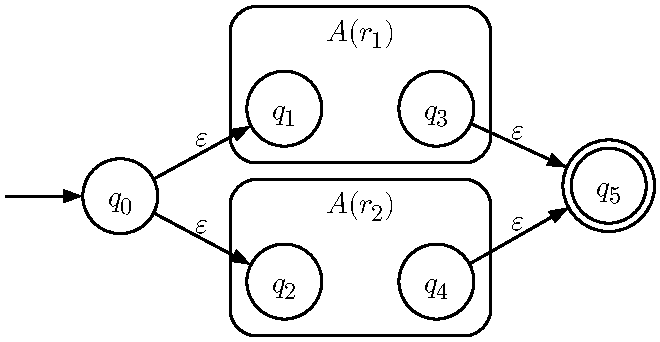
\includegraphics[scale=0.8]{Abbildungen/aPlus.pdf}
      \caption{The \simtextsc{Nfa} $A(r_1 + r_2)$.}
      \label{fig:aPlus.eps}
      \end{figure}
      Figure \ref{fig:aPlus.eps} shows the \simtextsc{Nfa} $A(r_1 + r_2)$.
      In addition to the states of $A(r_1)$ and $A(r_2)$ there are two more states:
      \begin{enumerate}
      \item $q_0$ is the start state of the \simtextsc{Nfa} $A(r_1 + r_2)$,
      \item $q_5$ is the only accepting state of the \simtextsc{Nfa} $A(r_1 + r_2)$.
      \end{enumerate}
      In addition to the transitions of $A(r_1)$ and $A(r_2)$ the \simtextsc{Nfa} $A(r_1+r_2)$
      has four more $\varepsilon$-transitions.
      \begin{enumerate}
      \item The new start state $q_0$ has two
            $\varepsilon$-transitions leading to the start states $q_1$ and $q_2$ of the \simtextsc{Nfa}s
            $A(r_1)$ and $A(r_2)$.
      \item Each of the accepting states $q_3$ and $q_4$ of the \simtextsc{Nfa}s
             $A(r_1)$ and $A(r_2)$ has an $\varepsilon$-transition to the new accepting state $q_5$.
      \end{enumerate}
      In order to simplify this \simtextsc{Nfa} we could identify the three states
      $q_0$, $q_1$ and $q_2$ and the three states $q_3$, $q_4$ and $q_5$.  However, the resulting \simtextsc{Nfa}
      would be more difficult to understand and hence we are \underline{\red{not}} doing this when creating 
      \simtextsc{Nfa}s by hand.
\item In order to define the \simtextsc{Nfa} $A(r^*)$ we assume that we have already constructed an
      \simtextsc{Nfa} $A(r)$ such that $L\bigl(A(r)\bigr) = L(r)$ and that $A(r)$ has the form
      \\[0.2cm]
      \hspace*{1.3cm}
      $A(r) = \bigl\langle Q, \Sigma, \delta, q_1, \{ q_2 \} \bigr\rangle$.
      \\[0.2cm]
      Then  $A(r^*)$ is defined as follows:
      \\[0.2cm]
      \hspace*{0.8cm}
       $\bigl\langle \{ q_0, q_3 \} \cup Q, \Sigma, 
                \bigl\{ \pair(q_0,\varepsilon) \mapsto \{q_1, q_3\}, \pair(q_2,\varepsilon) \mapsto \{q_1, q_3\} \bigr\} 
                \cup \delta, q_0, \{ q_3 \} \bigr\rangle$.
      \\[0.2cm]


      \begin{figure}[!ht]
        \centering
      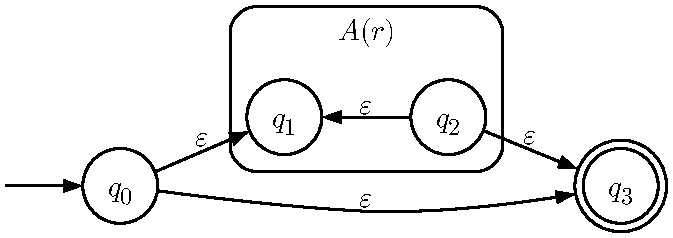
\includegraphics[scale=0.8]{Abbildungen/aStar.pdf}
      \caption{The \simtextsc{Nfa} $A(r^*)$.}
      \label{fig:aStar.eps}
      \end{figure}
      Figure \ref{fig:aStar.eps} shows the \simtextsc{Nfa} $A(r^*)$.
      In comparison with $A(r)$ this \simtextsc{Nfa} has two additional states.
      \begin{enumerate}
      \item $q_0$ is the start state of $A(r^*)$,
      \item $q_3$ is the only accepting state of $A(r^*)$.
      \end{enumerate}
      The \simtextsc{Nfa} $A(r^*)$ has four more $\varepsilon$-transitions than $A(r)$: 
      \begin{enumerate}
      \item The new start state  $q_0$ has $\varepsilon$-transitions to the states
            $q_1$ and $q_3$.
      \item $q_2$ has an $\varepsilon$-transition back to the state $q_1$.
      \item $q_2$ also has an $\varepsilon$-transition to the state $q_3$.
      \end{enumerate}
      \textbf{\textcolor{red}{Attention}}:  If we would identify the two states 
      $q_0$ and $q_1$ and the two states $q_2$ and $q_3$, then the resulting \simtextsc{Nfa} would no longer be
      correct!
\end{enumerate}

\exerciseEng
Construct an \simtextsc{Nfa} for the regular expression
\\[0.2cm]
\hspace*{1.3cm}
$(\texttt{a} + \texttt{b}) \cdot \texttt{a}^* \cdot \texttt{b}$.  
\eox

\subsection{Implementation}
The \textsl{Jupyter notebook} 
\\[0.2cm]
\hspace*{1.3cm}
\href{https://github.com/karlstroetmann/Formal-Languages/blob/master/Python/Chapter-04-05/03-Regexp-2-NFA.ipynb}{\texttt{Python/Chapter-04-05/03-Regexp-2-NFA.ipynb}} 
\\[0.2cm]
implements the theory discussed in this section.  It represents regular expressions as nested tuples:
\begin{enumerate}
\item The regular expression $\emptyset$ is represented by the number \texttt{0}.
\item The regular expression $\varepsilon$ is represented by the string \texttt{'𝜀'}.
\item A character $c \in \Sigma$ is represented by the string \texttt{'$c$'}.
\item If the regular expressions $r_1$ and $r_2$ are represented by the values $v_1$ and $v_2$, then
      \begin{enumerate}
      \item $r_1 \cdot r_2$ is represented by the triple \texttt{(}$v_1$\texttt{, '⋅', }$v_2$\texttt{)},
      \item $r_1 + r_2$ is represented by the triple \texttt{(}$v_1$\texttt{, '+', }$v_2$\texttt{)}, and
      \item $r_1^*$ is represented by the pair \texttt{(}$v_1$\texttt{, '*')}.
      \end{enumerate}
\end{enumerate}
For example, the regular expression $(\texttt{a} + \texttt{b}) \cdot \texttt{a}^*$ is represented by the nested
tuple
\\[0.2cm]
\hspace*{1.3cm}
\texttt{(('a', '+', 'b'), '⋅', ('a', '*'))}.
\\[0.2cm]
The notebook
\href{https://github.com/karlstroetmann/Formal-Languages/blob/master/Python/Chapter-04-05/RegExp-Parser.ipynb}{\texttt{RegExp-Parser.ipynb}}
provides the function \texttt{parse}, which turns a string like \texttt{'(a+b)a*'} into this representation.

The notebook \texttt{03-Regexp-2-NFA} implements the construction of $A(r)$ as the methods of the class
\texttt{RegExp2NFA}.  It defines most of these methods as functions in cells of their own.  The line
\\[0.2cm]
\hspace*{1.3cm}
\texttt{@method\_of(RegExp2NFA)}
\\[0.2cm]
in front of the definition of such a function makes this function a method of the class \texttt{RegExp2NFA}.
The listings omit these lines and the declarations of these methods in the body of the class, which are only
needed by the type checker.

\begin{figure}[!ht]
\centering
\begin{minted}[ frame         = lines,
                framesep      = 0.3cm,
                firstnumber   = 1,
                bgcolor       = sepia,
                numbers       = left,
                numbersep     = 0.3cm,
                xleftmargin   = 0.5cm,
                xrightmargin  = 0.5cm,
                gobble        = 4,
              ]{python3}
    class RegExp2NFA:
        def __init__(self, Sigma):
            self.Sigma      = Sigma
            self.StateCount = 0

    def getNewState(self):
        self.StateCount += 1
        return self.StateCount

    def toNFA(self, r):
        match r:
            case 0:
                return self.genEmptyNFA()
            case '𝜀':
                return self.genEpsilonNFA()
            case r if isinstance(r, str) and len(r) == 1:
                return self.genCharNFA(r)
            case (r1, '⋅', r2):
                return self.catenate(self.toNFA(r1), self.toNFA(r2))
            case (r1, '+', r2):
                return self.disjunction(self.toNFA(r1),
                                        self.toNFA(r2))
            case (r1, '*'):
                return self.kleene(self.toNFA(r1))
            case _:
                raise ValueError(
                    f'{r} is not a proper regular expression.')
\end{minted}
\vspace*{-0.3cm}
\caption{The class \texttt{RegExp2NFA} and the methods \texttt{getNewState} and \texttt{toNFA}.}
\label{fig:03-Regexp-2-NFA.ipynb:toNFA}
\end{figure}

\noindent
Figure \ref{fig:03-Regexp-2-NFA.ipynb:toNFA} on page \pageref{fig:03-Regexp-2-NFA.ipynb:toNFA} shows the class
\texttt{RegExp2NFA} together with the methods \texttt{getNewState} and \texttt{toNFA}.
\begin{enumerate}
\item Line 1 -- 4 define the class \texttt{RegExp2NFA}.  The member variable \texttt{Sigma} stores the alphabet
      $\Sigma$, which is a component of every \simtextsc{Nfa} that is constructed.  The member variable
      \texttt{StateCount} counts the states that have been created so far.
\item Line 6 -- 8 define the method \texttt{getNewState}, which returns a new number every time it is called.
      The construction of $A(r_1 \cdot r_2)$ and $A(r_1 + r_2)$ assumes that the sets of states of $A(r_1)$ and
      $A(r_2)$ are disjoint.  The implementation achieves this without renaming any states:  Every state is
      created by the method \texttt{getNewState}.  Hence no state is created twice and different
      \simtextsc{Nfa}s that have been constructed by the same object have disjoint sets of states.
\item Line 10 -- 27 define the method \texttt{toNFA}, which computes $A(r)$ by recursion on the regular
      expression $r$.  It uses a \texttt{match} statement.  \blue{Structural pattern matching}\index{pattern
      matching} is the natural way to work with values that are represented as nested tuples:  The
      \texttt{match} statement compares the value \texttt{r} with the patterns that follow the keyword
      \texttt{case}, one after another, and executes the code of the first pattern that matches.
      \begin{enumerate}
      \item Line 12 -- 13 handle the regular expression $\emptyset$, since the pattern \texttt{0} matches only the
            number \texttt{0}.  Similarly, line 14 -- 15 handle the regular expression $\varepsilon$.
      \item The pattern \texttt{r} in line 16 matches every value and binds it to the variable \texttt{r}.
            However, it is followed by a \blue{guard}\index{pattern matching!guard}, i.e.~a condition that starts
            with the keyword \texttt{if}.  The case is only chosen if this condition is true, i.e.~if
            \texttt{r} is a string of length one.  Then line 17 constructs the \simtextsc{Nfa} $A(c)$ for the
            character $c$ = \texttt{r}.  As the string \texttt{'𝜀'} has length one, too, the order of the cases
            matters:  The case in line 14 has to precede the case in line 16.
      \item The pattern in line 18 matches every triple whose second component is the string \texttt{'⋅'}.  It
            binds the first and the third component of the triple to the variables \texttt{r1} and \texttt{r2}.
            Line 19 computes the \simtextsc{Nfa}s $A(r_1)$ and $A(r_2)$ recursively and combines them into the
            \simtextsc{Nfa} $A(r_1 \cdot r_2)$.  Line 20 -- 22 handle the regular expression $r_1 + r_2$ in the
            same way, while line 23 -- 24 construct the \simtextsc{Nfa} $A(r_1^*)$ for a pair whose second
            component is the string \texttt{'*'}.
      \item The pattern \texttt{\_} in line 25 matches every value.  As this case is only reached if the value
            \texttt{r} does not represent a regular expression, line 26 -- 27 raise an exception.
      \end{enumerate}
\end{enumerate}

\begin{figure}[!ht]
\centering
\begin{minted}[ frame         = lines,
                framesep      = 0.3cm,
                firstnumber   = 1,
                bgcolor       = sepia,
                numbers       = left,
                numbersep     = 0.3cm,
                xleftmargin   = 0.5cm,
                xrightmargin  = 0.5cm,
                gobble        = 4,
              ]{python3}
    def genEmptyNFA(self):
        q0 = self.getNewState()
        q1 = self.getNewState()
        return {q0, q1}, self.Sigma, {}, q0, { q1 }

    def genEpsilonNFA(self):
        q0 = self.getNewState()
        q1 = self.getNewState()
        delta = { (q0, '𝜀'): {q1} }
        return {q0, q1}, self.Sigma, delta, q0, { q1 }

    def genCharNFA(self, c):
        q0 = self.getNewState()
        q1 = self.getNewState()
        delta = { (q0, c): {q1} }
        return {q0, q1}, self.Sigma, delta, q0, { q1 }
\end{minted}
\vspace*{-0.3cm}
\caption{The methods \texttt{genEmptyNFA}, \texttt{genEpsilonNFA}, and \texttt{genCharNFA}.}
\label{fig:03-Regexp-2-NFA.ipynb:genEmptyNFA}
\end{figure}

\noindent
Figure \ref{fig:03-Regexp-2-NFA.ipynb:genEmptyNFA} on page \pageref{fig:03-Regexp-2-NFA.ipynb:genEmptyNFA} shows
the methods that construct the \simtextsc{Nfa}s $A(\emptyset)$, $A(\varepsilon)$, and $A(c)$.  Each of them creates
two new states:  The start state $q_0$ and the accepting state $q_1$.  The \simtextsc{Nfa} $A(\emptyset)$ has no
transitions at all.  Therefore, its transition function is the empty dictionary \texttt{\{\}} in line 4.  Note that
in \textsl{Python}, the expression \texttt{\{\}} denotes an empty dictionary, while the empty set is written as
\texttt{set()}.  The \simtextsc{Nfa}s $A(\varepsilon)$ and $A(c)$ have a single transition from $q_0$ to $q_1$,
which is labelled with $\varepsilon$ and the character $c$, respectively.

\begin{figure}[!ht]
\centering
\begin{minted}[ frame         = lines,
                framesep      = 0.3cm,
                firstnumber   = 1,
                bgcolor       = sepia,
                numbers       = left,
                numbersep     = 0.3cm,
                xleftmargin   = 0.5cm,
                xrightmargin  = 0.5cm,
                gobble        = 4,
              ]{python3}
    def catenate(self, f1, f2):
        M1, Sigma, delta1, q1, A1 = f1
        M2, Sigma, delta2, q3, A2 = f2
        q2, = A1 # extract the element from the set A1
        delta = delta1 | delta2
        delta[q2, '𝜀'] = {q3}
        return M1 | M2, Sigma, delta, q1, A2

    def disjunction(self, f1, f2):
        Q1, Sigma, delta1, q1, A1 = f1
        Q2, Sigma, delta2, q2, A2 = f2
        q3, = A1
        q4, = A2
        q0 = self.getNewState()
        q5 = self.getNewState()
        delta = delta1 | delta2
        delta[q0, '𝜀'] = { q1, q2 }
        delta[q3, '𝜀'] = { q5 }
        delta[q4, '𝜀'] = { q5 }
        return { q0, q5 } | Q1 | Q2, Sigma, delta, q0, { q5 }

    def kleene(self, f):
        Q, Sigma, delta0, q1, A = f
        q2, = A
        q0 = self.getNewState()
        q3 = self.getNewState()
        delta = delta0 | {}    # copy delta0, so that f is not changed
        delta[q0, '𝜀'] = { q1, q3 }
        delta[q2, '𝜀'] = { q1, q3 }
        return { q0, q3 } | Q, Sigma, delta, q0, { q3 }
\end{minted}
\vspace*{-0.3cm}
\caption{The methods \texttt{catenate}, \texttt{disjunction}, and \texttt{kleene}.}
\label{fig:03-Regexp-2-NFA.ipynb:catenate}
\end{figure}

\noindent
Figure \ref{fig:03-Regexp-2-NFA.ipynb:catenate} on page \pageref{fig:03-Regexp-2-NFA.ipynb:catenate} shows the
methods that construct the \simtextsc{Nfa}s $A(r_1 \cdot r_2)$, $A(r_1 + r_2)$, and $A(r^*)$.  They use the same
names for the states as the definitions given above.
\begin{enumerate}
\item Line 1 -- 7 define the method \texttt{catenate}, which computes $A(r_1 \cdot r_2)$ from the
      \simtextsc{Nfa}s \texttt{f1} = $A(r_1)$ and \texttt{f2} = $A(r_2)$.
      \begin{enumerate}
      \item Line 2 -- 3 extract the components of these \simtextsc{Nfa}s.  Both have the same alphabet.
      \item The set \texttt{A1} of accepting states of $A(r_1)$ contains exactly one element.  The assignment in
            line 4 extracts this element:  Because of the comma, the left hand side is a tuple with one
            component, and the set on the right hand side is unpacked into this tuple.  The assignment fails
            if the set does not contain exactly one element.
      \item For dictionaries, the operator ``\texttt{|}'' in line 5 creates a new dictionary that contains the
            entries of both dictionaries.  As the sets of states of $A(r_1)$ and $A(r_2)$ are disjoint, the two
            dictionaries have no key in common.  As the dictionary is new, line 6 does not change the
            transition function of $A(r_1)$.
      \item Line 6 adds the $\varepsilon$-transition from $q_2$ to $q_3$.  As $A(r_1)$ has no transitions out
            of its accepting state $q_2$, no transition of $A(r_1)$ is overwritten.
      \item Line 7 returns $A(r_1 \cdot r_2)$.  The operator ``\texttt{|}'' computes the union of the two sets
            of states.  The start state is the start state $q_1$ of $A(r_1)$, and the set of accepting states is
            the set $\{ q_4 \}$ of $A(r_2)$.
      \end{enumerate}
\item Line 9 -- 20 define the method \texttt{disjunction}, which computes $A(r_1 + r_2)$.  Line 14 -- 15
      create the new start state $q_0$ and the new accepting state $q_5$, and line 17 -- 19 add the four
      $\varepsilon$-transitions.
\item Line 22 -- 30 define the method \texttt{kleene}, which computes $A(r^*)$ from the \simtextsc{Nfa}
      \texttt{f} = $A(r)$.  Line 27 copies the transition function of $A(r)$, since otherwise line 28 -- 29
      would change it.  In the methods \texttt{catenate} and \texttt{disjunction}, such a copy is not needed,
      since the operator ``\texttt{|}'' creates a new dictionary anyway.  Line 29 adds the
      $\varepsilon$-transitions from the accepting state $q_2$ of $A(r)$ back to its start state $q_1$ and to the
      new accepting state $q_3$.
\end{enumerate}
The notebook
\href{https://github.com/karlstroetmann/Formal-Languages/blob/master/Python/Chapter-04-05/04-Test-Regexp-2-NFA.ipynb}{\texttt{04-Test-Regexp-2-NFA.ipynb}}
constructs a \simtextsc{Nfa} for the regular expression $\texttt{a}^* \cdot \texttt{b} \cdot \texttt{a}^*$,
transforms it into a \simtextsc{Dfa} with the function \texttt{nfa2dfa}, and draws both finite state machines.


\section{Translating a \textsc{DFA} into a Regular Expression}
In this last section we start with a \simtextsc{Dfa} $F$ and construct a regular expression $r$
such that we have
\\[0.2cm]
\hspace*{1.3cm}
$L(r) = L(F)$. 
\\[0.2cm]
We assume that the \simtextsc{Dfa} $F$ is given as follows:
\\[0.2cm]
\hspace*{1.3cm}
$F = \bigl\langle \{ q_0, q_1, \cdots, q_n \}, \Sigma, \delta, q_0, A \bigr\rangle$.
\\[0.2cm]
For every pair of states $\pair(p_1,p_2) \in Q \times Q$ we define a regular expression
$r(p_1, p_2)$ such that $r(p_1, p_2)$ describes those strings $w$ that take the \simtextsc{Dfa} $F$ from the state
$p_1$ to the state $p_2$, i.e.~we have
\\[0.2cm]
\hspace*{1.3cm}
$L\bigl(r(p_1, p_2)\bigr) = 
  \bigl\{ w \in \Sigma^* \mid \pair(p_1,w) \leadsto^* \pair(p_2, \lambda) \bigr\}$.
\\[0.2cm]  
The definition of $r(p_1, p_2)$ is done by first defining auxiliary regular expressions 
$r^{(k)}(p_1, p_2)$ for all $k =0,\cdots,n+1$.   The regular expression $r^{(k)}(p_1, p_2)$ specifies those
strings that take the \simtextsc{Dfa} $F$ from the state
$p_1$ to the state $p_2$ while only visiting states from the set
\\[0.2cm]
\hspace*{1.3cm}
$Q_k := \bigl\{ q_i \mid i \in \{0,\cdots,k-1 \}  \bigr\}$
\\[0.2cm]
in between.  Observe that
\\[0.2cm]
\hspace*{1.3cm}
$Q_0 = \{\}$ \quad and \quad $Q_{n+1} = \{q_0, \cdots, q_n \} = Q$.
\\[0.2cm]
To this end we define the ternary relation
\\[0.2cm]
\hspace*{1.3cm}
$\mapsto_k \;\subseteq\; (Q \times \Sigma^* \times Q)$.
\\[0.2cm]
Given two states $p, q \in Q$ and a string $w$ we have that
\\[0.2cm]
\hspace*{1.3cm}
$p \stackrel{w}{\mapsto}_k q$
\\[0.2cm]
holds iff the \simtextsc{Dfa} $F$ switches from the state $p$ to the state $q$ when it reads the string $w$
but on reading $w$ only visits states from the set
$Q_k$ \blue{in-between}.  Here, ``in-between'' specifies that the states $p$ and $q$ may well be outside of the set
$Q_k$, only the states between $p$ and $q$ are required to be elements of $Q_k$.
The formal definition of $p \stackrel{w}{\mapsto}_k q$ is done by induction on  $w$:
\begin{enumerate}
\item[B.C.:] $|w| \leq 1$.  Then there are two cases:
  \begin{enumerate}
  \item $p \stackrel{\lambda}{\mapsto}_k p$,

        because when the empty string is read we can only reach the state $p$ if we start in the state $p$.
  \item $\delta(p, c) = q \;\Rightarrow\; p \stackrel{c}{\mapsto}_k q$,

        because when the \simtextsc{Dfa} reads the character $c$ and switches from state $p$ directly
        to the state $q$, there are no states ``inbetween''.
  \end{enumerate}
\item[I.S.:] $w = cv$ where $|v| \geq 1$.

             Here we have:
             \hspace*{1.3cm}
            $p \stackrel{c}{\mapsto} q \wedge q \in Q_k \wedge q \stackrel{v}{\mapsto}_k r
              \;\Rightarrow\; p \stackrel{cv}{\mapsto}_k r$.
\end{enumerate}
Now we are ready to define the regular expressions $r^{(k)}(p_1, p_2)$ for all $k=0,\cdots,n+1$.
This definition will be done such that we have
\\[0.2cm]
\hspace*{1.3cm}
$L\bigl(r^{(k)}(p_1, p_2)\bigr) = \bigl\{ w \in \Sigma^* \mid p_1 \stackrel{w}{\mapsto}_k p_2 \bigr\}$.
\\[0.2cm]
The definition of the regular expressions $r^{(k)}(p_1, p_2)$ is done by induction on $k$.
\begin{enumerate}
\item[B.C.:] $k = 0$.  

  Then we have $Q_0 = \{\}$.
  Therefore, when the \simtextsc{Dfa} switches from the state $p_1$ to the state $p_2$ it must not visit any
  states in-between.  There are two cases.
  \begin{enumerate}
  \item $p_1 \not= p_2$:  Then we can have  $p_1 \stackrel{w}{\mapsto}_0 p_2$ only if $w$ contains but a
        single letter.  Define
        \\[0.2cm]
        \hspace*{1.3cm}
        $\{ c_1, \cdots, c_l \} := \{ c \in \Sigma \mid \delta(p_1,c) = p_2 \}$
        \\[0.2cm]
        as the set of all letters that take the \simtextsc{Dfa} from the state $p_1$ to the state $p_2$.
        If this set is not empty we define 
        \\[0.2cm]
        \hspace*{1.3cm}
        $r^{(0)}(p_1, p_2) := c_1 + \cdots + c_l$. 
        \\[0.2cm]
        If this set is empty, then there is no direct transition from  $p_1$ to $p_2$ and we define
        \\[0.2cm]
        \hspace*{1.3cm}
        $r^{(0)}(p_1, p_2) := \emptyset$.
  \item $p_1 = p_2$:  Again we define
        \\[0.2cm]
        \hspace*{1.3cm}
        $\{ c_1, \cdots, c_l \} := \{ c \in \Sigma \mid \delta(p_1,c) = p_1 \}$.
        \\[0.2cm]
        If this set is not empty we have
        \\[0.2cm]
        \hspace*{1.3cm}
        $r^{(0)}(p_1, p_1) := c_1 + \cdots + c_l + \varepsilon$.
        \\[0.2cm]
        Otherwise we have
        \\[0.2cm]
        \hspace*{1.3cm}
        $r^{(0)}(p_1, p_1) := \varepsilon$.
   \end{enumerate}
\item[I.S.:] $k \mapsto k+1$.  

  We have that
  \\[0.2cm]
  \hspace*{1.3cm}
  $Q_{k+1} = Q_k \cup \{q_k\}$
  \\[0.2cm]
  Therefore, when compared to the regular expression $r^{(k)}(p_1, p_2)$,
  the regular expression  $r^{(k+1)}(p_1, p_2)$ describes strings that cause the \simtextsc{Dfa} to potentially
  visit the state  $q_k$ in addition to the states from the set $Q_k$.
  If the \simtextsc{Dfa} reads a string $w$ that switches the state $p_1$ to the state $p_2$ while only using states
  from the set $Q_{k+1}$, then there are two cases.
  \begin{enumerate}
  \item We already have $p_1 \stackrel{w}{\mapsto}_k p_2$, i.e. the DFA uses only states from $Q_k$ and the
        state $q_{k}$ isn't used.
  \item The string $w$ can be written as  $w = w_1 s_1\cdots s_l w_2$ where we have:
        \begin{itemize}
        \item $p_1 \stackrel{w_1}{\mapsto}_k q_k$,
        \item $q_k \stackrel{s_i}{\mapsto}_k q_k$ \quad for all $i \in \{ 1, \cdots, l\}$,
        \item $q_k \stackrel{w_2}{\mapsto}_k p_2$.
        \end{itemize}
        Therefore we define
        \\[0.2cm]
        \hspace*{1.3cm}
        $r^{(k+1)}(p_1,p_2) := 
         r^{(k)}(p_1,p_2) + 
         r^{(k)}(p_1,q_k) \cdot \bigl(r^{(k)}(q_k,q_k)\bigr)^* \cdot r^{(k)}(q_k,p_2)$.
  \end{enumerate}  
\end{enumerate}
Now we are ready to define the regular expressions $r(p_1,p_2)$ for all states $p_1$ and $p_2$:
\\[0.2cm]
\hspace*{1.3cm}
$r(p_1,p_2) := r^{(n+1)}(p_1,p_2)$. 
\\[0.2cm]
This regular expression specifies all strings that take the \simtextsc{Dfa} from the state
$p_1$ to the state $p_2$ while using any state from the set 
$Q_{n+1}$ in-between.   Since we have
\\[0.2cm]
\hspace*{1.3cm}
$Q_{n+1} = \bigl\{ q_0, \cdots, q_n \bigr\} = Q$
\\[0.2cm]
we can use any state in-between.

In order to construct a regular expression that specifies the language accepted by a \simtextsc{Dfa}
$F$ we write the set $A$ of accepting states of $F$ as
\\[0.2cm]
\hspace*{1.3cm}
$A = \{ t_1, \cdots, t_m \}$.
\\[0.2cm]
Then the regular expression $r(F)$ is defined as
\\[0.2cm]
\hspace*{1.3cm}
$r(F) := r(q_0, t_1) + \cdots + r(q_0, t_m)$.
\\[0.2cm]
This regular expression specifies those strings that take the \simtextsc{Dfa} $F$ from its start state $q_0$ into
any of its accepting states.  If $F$ has no accepting states at all, then $F$ does not accept any string and
we define $r(F) := \emptyset$.
\eox


\exerciseEng
Take the \simtextsc{Dfa} shown in Figure \ref{fig:abstara.dot} and construct an equivalent regular expression.


\solutionEng
The \simtextsc{Dfa} has two states: $0$ and $1$.  We start by computing the regular expressions
$r^{(k)}(i,j)$ for all $i,j\in\{0,1\}$ for  $k =0$, $1$, and $2$:
\begin{enumerate}
\item For $k = 0$ we have:
      \begin{enumerate}
      \item $r^{(0)}(0, 0) = \texttt{a} + \varepsilon$,
      \item $r^{(0)}(0, 1) = \texttt{b}$,
      \item $r^{(0)}(1, 0) = \emptyset$,
      \item $r^{(0)}(1, 1) = \texttt{a} + \varepsilon$.
      \end{enumerate}
\item For $k=1$ we have:
      \begin{enumerate}
      \item For $r^{(1)}(0, 0)$ we have:
            \begin{eqnarray*}
                  r^{(1)}(0, 0) 
            & = & r^{(0)}(0, 0) + 
                  r^{(0)}(0, 0) \cdot \bigl(r^{(0)}(0, 0)\bigr)^* \cdot r^{(0)}(0, 0) \\
            & \doteq & r^{(0)}(0, 0) \cdot \bigl(r^{(0)}(0, 0)\bigr)^*
            \end{eqnarray*}
             In the last step we used the fact that 
             \\[0.2cm]
             \hspace*{1.3cm}
             $
             \begin{array}[t]{lcl}
               r + r \cdot r^* \cdot r & \doteq & r \cdot (\varepsilon + r^* \cdot r) \\
                                       & \doteq & r \cdot r^*
             \end{array}
             $
             \\[0.2cm]
             to simplify the result.
             If we substitute for $r^{(0)}(0, 0)$ the expression $\texttt{a} + \varepsilon$  
             we get 
             \\[0.2cm]
             \hspace*{1.3cm}
             $r^{(1)}(0, 0) \doteq (\texttt{a} + \varepsilon)\cdot (\texttt{a} + \varepsilon)^*$.
             \\[0.2cm]
             As we have $(\texttt{a} + \varepsilon)\cdot (\texttt{a} + \varepsilon)^* \doteq \texttt{a}^*$ we have
             \\[0.2cm]
             \hspace*{1.3cm}
             $r^{(1)}(0, 0) \doteq \texttt{a}^*$.
      \item For $r^{(1)}(0, 1)$ we have:
            \begin{eqnarray*}
                  r^{(1)}(0, 1) 
            & \doteq & r^{(0)}(0, 1) + 
                  r^{(0)}(0, 0) \cdot \bigl(r^{(0)}(0, 0)\bigr)^* \cdot r^{(0)}(0, 1) \\
            & \doteq & \texttt{b} + 
                  (\texttt{a} + \varepsilon) \cdot (\texttt{a} + \varepsilon)^* \cdot \texttt{b} \\
            & \doteq & \texttt{b} + \texttt{a}^* \cdot \texttt{b} \\
            & \doteq & (\varepsilon + \texttt{a}^*) \cdot \texttt{b} \\
            & \doteq & \texttt{a}^* \cdot \texttt{b} 
        \end{eqnarray*}
      \item For $r^{(1)}(1, 0)$ we have:
            \begin{eqnarray*}
                  r^{(1)}(1, 0) 
            & \doteq & r^{(0)}(1, 0) + 
                  r^{(0)}(1, 0) \cdot \bigl(r^{(0)}(0, 0)\bigr)^* \cdot r^{(0)}(0, 0) \\
            & \doteq & \emptyset + \emptyset \cdot (\texttt{a} + \varepsilon)^* \cdot (\texttt{a} + \varepsilon) \\
            & \doteq & \emptyset
            \end{eqnarray*}
      \item For $r^{(1)}(1, 1)$ we have
            \begin{eqnarray*}
                  r^{(1)}(1, 1)
            & \doteq & r^{(0)}(1, 1) + 
                  r^{(0)}(1, 0) \cdot \bigl(r^{(0)}(0, 0)\bigr)^* \cdot r^{(0)}(0, 1) \\
            & \doteq & (\texttt{a} + \varepsilon) + 
                  \emptyset \cdot (\texttt{a} + \varepsilon)^* \cdot \texttt{b} \\
            & \doteq & (\texttt{a} + \varepsilon) + \emptyset  \\
            & \doteq & \texttt{a} + \varepsilon  
            \end{eqnarray*}
      \end{enumerate}
\item For $k=2$ we only have to compute the regular expression $r^{(2)}(0, 1)$:
            \begin{eqnarray*}
                  r^{(2)}(0, 1)
            & \doteq & r^{(1)}(0, 1) + 
                  r^{(1)}(0, 1) \cdot \bigl(r^{(1)}(1, 1)\bigr)^* \cdot r^{(1)}(1, 1) \\
            & \doteq & \texttt{a}^* \cdot \texttt{b} + 
                  \texttt{a}^* \cdot \texttt{b} \cdot (\texttt{a} + \varepsilon)^* \cdot (\texttt{a} + \varepsilon) \\
            & \doteq & \texttt{a}^* \cdot \texttt{b} + \texttt{a}^* \cdot \texttt{b} \cdot \texttt{a}^* \\
            & \doteq & \texttt{a}^* \cdot \texttt{b} \cdot (\varepsilon + \texttt{a}^*) \\
            & \doteq & \texttt{a}^* \cdot \texttt{b} \cdot \texttt{a}^*.
        \end{eqnarray*}
\end{enumerate}
As the state 0 is the start state and the state $1$ is the only accepting state we have
\\[0.2cm]
\hspace*{1.3cm}
$r(F) = r^{(2)}(0, 1) \doteq \texttt{a}^* \cdot \texttt{b} \cdot \texttt{a}^*$.
\qed


\exerciseEng
Take the \simtextsc{Dfa} shown in Figure \ref{fig:exercise-13.eps} on page
\pageref{fig:exercise-13.eps} and construct a regular expression specifying the same language as this
\simtextsc{Dfa}.
\vspace*{0.1cm}

\noindent
\textbf{Hint}: In order to avoid unnecessary computations, you should only compute those regular expressions
$r^{(k)}(p, q)$ that are needed in order to compute $r^{(3)}(q_0, q_2)$. 
\eox

\begin{figure}[!ht]
  \centering
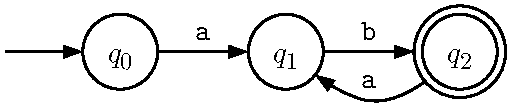
\includegraphics[scale=1.0]{Abbildungen/exercise-13.pdf}
\caption{A \simtextsc{Dfa}.}
\label{fig:exercise-13.eps}
\end{figure}

\subsection{Implementation}
The \textsl{Jupyter notebook} 
\\[0.2cm]
\hspace*{1.3cm}
\href{https://github.com/karlstroetmann/Formal-Languages/blob/master/Python/Chapter-04-05/05-DFA-2-RegExp.ipynb}{\texttt{Python/Chapter-04-05/05-DFA-2-RegExp.ipynb}}
\\[0.2cm]
contains a program that takes a  \simtextsc{Dfa} $F$ and computes a regular expression $r$ such that
$r$ specifies the language accepted by $F$, i.e.~we have $L(r) = L(F)$.  Figure
\ref{fig:05-DFA-2-RegExp.ipynb:rpq} on page \pageref{fig:05-DFA-2-RegExp.ipynb:rpq} shows the functions of this
notebook.

\begin{figure}[!ht]
\centering
\begin{minted}[ frame         = lines,
                framesep      = 0.3cm,
                firstnumber   = 1,
                bgcolor       = sepia,
                numbers       = left,
                numbersep     = 0.3cm,
                xleftmargin   = 0.5cm,
                xrightmargin  = 0.5cm,
                gobble        = 4,
              ]{python3}
    def regexp_sum(S):
        n = len(S)
        match n:
            case 0:
                return 0
            case 1:
                r, = S
                return r
            case _:
                r, *Rs = S
                return (r, '+', regexp_sum(Rs))

    def rpq(p1, p2, Σ, 𝛿, Allowed):
        if len(Allowed) == 0:
            AllChars = { c for c in Σ if 𝛿.get((p1, c)) == p2 }
            r = regexp_sum(AllChars)
            if p1 == p2:
                return ('𝜀', '+', r)
            else:
                return r
        else:
            q, *RestAllowed = Allowed
            rp1p2 = rpq(p1, p2, Σ, 𝛿, RestAllowed)
            rp1q  = rpq(p1,  q, Σ, 𝛿, RestAllowed)
            rqq   = rpq( q,  q, Σ, 𝛿, RestAllowed)
            rqp2  = rpq( q, p2, Σ, 𝛿, RestAllowed)
            return (rp1p2, '+', ((rp1q, '⋅', (rqq, '*')), '⋅', rqp2))

    def dfa_2_regexp(F):
        States, Σ, 𝛿, q0, Accepting = F
        r = regexp_sum({ rpq(q0, p, Σ, 𝛿, States)
                         for p in Accepting })
        return r
\end{minted}
\vspace*{-0.3cm}
\caption{The functions \texttt{regexp\_sum}, \texttt{rpq}, and \texttt{dfa\_2\_regexp}.}
\label{fig:05-DFA-2-RegExp.ipynb:rpq}
\end{figure}

\begin{enumerate}
\item Line 1 -- 11 define the function \texttt{regexp\_sum}.  Given a collection $S = \{ r_1, \cdots, r_n \}$ of
      regular expressions, it returns the regular expression $r_1 + \cdots + r_n$.
      \begin{enumerate}
      \item If $S$ is empty, the sum is empty and line 5 returns the regular expression $\emptyset$, which is
            represented by the number \texttt{0}.
      \item If $S$ has exactly one element, line 7 extracts this element in the same way as the method
            \texttt{catenate} in Figure \ref{fig:03-Regexp-2-NFA.ipynb:catenate} extracts the accepting state.
      \item Otherwise, the assignment in line 10 assigns the first element of $S$ to the variable \texttt{r}.
            Because of the operator ``\texttt{*}'', the variable \texttt{Rs} collects the remaining elements
            in a list.  Hence the recursive call in line 11 receives a list instead of a set.  The result has
            the form $r_1 + \bigl(r_2 + (\cdots + r_n)\bigr)$.  For a set, the order of the elements is not
            specified.  However, this order does not matter, since the operator ``$+$'' is commutative with
            respect to the languages that the regular expressions describe.
      \end{enumerate}
\item Line 13 -- 27 define the function \texttt{rpq}, which computes the regular expressions
      $r^{(k)}(p_1, p_2)$.  The definition of these regular expressions numbers the states of $F$ as
      $q_0, \cdots, q_n$ and allows only the states of the set $Q_k = \{ q_0, \cdots, q_{k-1} \}$ in-between.  The
      function \texttt{rpq} does not need to number the states.  Instead, its argument \texttt{Allowed} is the
      set of the states that are allowed in-between.  Hence we have
      \\[0.2cm]
      \hspace*{1.3cm}
      $\texttt{rpq}(p_1, p_2, \Sigma, \delta, Q_k) = r^{(k)}(p_1, p_2)$.
      \begin{enumerate}
      \item Line 14 -- 20 handle the case $\texttt{Allowed} = \{\}$, which corresponds to the case $k = 0$.
            Line 15 computes the set of all characters $c$ such that $\delta(p_1, c) = p_2$.  If the
            dictionary $\delta$ has no entry for the pair $\pair(p_1, c)$, the method \texttt{get} returns the
            value \texttt{None}, which is different from every state.  Therefore, the \simtextsc{Dfa} need not be
            complete.  Line 16 combines these characters with the operator ``$+$''.  If $p_1 = p_2$, the empty
            string takes $F$ from $p_1$ to $p_2$, too.  Therefore, line 18 adds the regular expression
            $\varepsilon$.  If there is no character $c$ such that $\delta(p_1, c) = p_1$, the result is the
            regular expression $\varepsilon + \emptyset$, which is equivalent to $\varepsilon$.
      \item Otherwise, line 22 splits the collection \texttt{Allowed} into a state $q$ and the list
            \texttt{RestAllowed} of the remaining states.  The state $q$ plays the role of the state $q_k$,
            while \texttt{RestAllowed} plays the role of the set $Q_k$.  Therefore, line 23 -- 26 compute the
            regular expressions $r^{(k)}(p_1, p_2)$, $r^{(k)}(p_1, q_k)$, $r^{(k)}(q_k, q_k)$, and
            $r^{(k)}(q_k, p_2)$ recursively, and line 27 returns the regular expression
            \\[0.2cm]
            \hspace*{1.3cm}
            $r^{(k)}(p_1,p_2) + r^{(k)}(p_1,q_k) \cdot \bigl(r^{(k)}(q_k,q_k)\bigr)^* \cdot r^{(k)}(q_k,p_2)$.
      \end{enumerate}
      Every call of \texttt{rpq} with a collection \texttt{Allowed} of $k > 0$ states makes four recursive calls
      with $k-1$ states.  Hence, if $F$ has $n$ states, the number of calls and the size of the resulting
      regular expression grow like $4^n$.  Therefore, this algorithm is only suitable for small
      \simtextsc{Dfa}s.
\item Line 29 -- 33 define the function \texttt{dfa\_2\_regexp}, which computes the regular expression
      \\[0.2cm]
      \hspace*{1.3cm}
      $r(F) = r(q_0, t_1) + \cdots + r(q_0, t_m)$,
      \\[0.2cm]
      where $\{ t_1, \cdots, t_m \}$ is the set of accepting states and all states are allowed in-between.  If
      $F$ has no accepting states, the function \texttt{regexp\_sum} returns the regular expression $\emptyset$.
\end{enumerate}
The notebook
\href{https://github.com/karlstroetmann/Formal-Languages/blob/master/Python/Chapter-04-05/06-Test-DFA-2-RegExp.ipynb}{\texttt{06-Test-DFA-2-RegExp.ipynb}}
applies the function \texttt{dfa\_2\_regexp} to a \simtextsc{Dfa} with three states.  As the resulting regular
expression is nearly unreadable, it is simplified with the function \texttt{simplify} from the notebook
\href{https://github.com/karlstroetmann/Formal-Languages/blob/master/Python/Chapter-04-05/Simplify.ipynb}{\texttt{Simplify.ipynb}}.

\section{Minimization of Finite State Machines}
In this section we show how to minimize the number of states of a \simtextsc{Dfa}
\\[0.2cm]
\hspace*{1.3cm}
$F = \langle Q, \Sigma, \delta, q_0, A \rangle$.
\\[0.2cm]
Without loss of generality we want to assume that the \simtextsc{Dfa} $F$ is complete: Therefore, we assume that
for each state $q \in Q$ and each letter $c \in \Sigma$ the expression $\delta(q, c)$ 
returns a state of $Q$.  Our goal is to find a complete \simtextsc{Dfa}
\\[0.2cm]
\hspace*{1.3cm}
$\mathtt{Min}(F) := \bigl\langle \mathcal{Q}_\sim, \Sigma, \Delta, [q_0]_\sim, \widehat{A} \,\bigr\rangle$
\\[0.2cm]
which accepts the same language as  $F$, so we have 
\\[0.2cm]
\hspace*{1.3cm}
$L\bigl(\mathtt{Min}(F)\bigr) = L(F)$
\\[0.2cm]
and for which the number of states of the set $\mathcal{Q}_\sim$ is minimal.  You might be wondering about the
meaning associated with $\mathcal{Q}_\sim$ and $[q_0]_\sim$:  We will introduce an \blue{equivalence
relation}\footnote{A binary relation $R \subseteq M \times M$ is an \blue{equivalence relation} on $M$ iff it has the
  following properties:
  \begin{enumerate}[(a)]
  \item $R$ is \blue{reflexive} on $M$, i.e.~$\forall x\in M: \langle x, x\rangle \in R$.
  \item $R$ is \blue{symmetric}, i.e.
    $\forall x,y\in M:\bigl(\langle x, y\rangle \in R \rightarrow \langle y, x\rangle\in R\bigr)$.
  \item $R$ is \blue{transitive}, i.e. $\forall x,y,z \in M:\bigl(\langle x, y\rangle \in R \wedge \langle
    y, z\rangle \in R \rightarrow \langle x, z\rangle \in R\bigr)$.
  \end{enumerate}}
$\sim$ on the set of states $Q$.  Basically, $p_1, p_2\in Q$ are \blue{equivalent}\index{equivalent states}\glsadd{sim} if they serve the same
purpose in the \simtextsc{Dfa} $F$, whatever that means.  If $p_1$ and $p_2$ are equivalent, this will be written as
\\[0.2cm]
\hspace*{1.3cm}
$p_1 \sim p_2$.
\\[0.2cm]
Given a state $p \in Q$, the \blue{equivalence class}\index{equivalence class}\glsadd{eqclass} of $p$ w.r.t.~the relation $\sim$, written $[p]_\sim$ is the set of all states that
are equivalent to $p$, i.e.~we have
\\[0.2cm]
\hspace*{1.3cm}
$[p]_\sim := \{ q \in Q \mid p \sim q \}$.
\\[0.2cm]
The new states of the \simtextsc{Dfa} $\texttt{Min}(F)$ will be equivalence classes of the equivalence relation
$\sim$.  Therefore we have
\\[0.2cm]
\hspace*{1.3cm}
$\mathcal{Q}_\sim := \bigl\{ [q]_\sim \;\big|\; q \in Q \bigr\}$.
\\[0.2cm]
The new start state $[q_0]_\sim$ is the set of all states that are equivalent to the state $q_0$.  The formal definitions of the
equivalence relation $\sim$, the function $\Delta: \mathcal{Q}_\sim \times \Sigma \rightarrow \mathcal{Q}_\sim$
and the set $\widehat{A}$ will be given later.

We start with the function 
\\[0.2cm]
\hspace*{1.3cm}
$\delta^*: Q \times \Sigma^* \rightarrow Q$
\\[0.2cm]
which extends the function $\delta$ by accepting a string instead of a single character as its second argument.
The function call $\delta^*(q,s)$ calculates the state $p$ which the \simtextsc{Dfa} $F$ enters if it reads the
string $s$ in the state $q$. As we have assumed the \simtextsc{Dfa} $F$ to be complete, we have that
\\[0.2cm]
\hspace*{1.3cm}
$\delta(q, c) \not= \Omega$ \quad for all $q \in Q$ and all $c \in \Sigma$ 
\\[0.2cm]
and then $\delta^*(q,w)$ is defined by induction on $w$ as follows:
\begin{enumerate}[(a)]
\item $\delta^*(q, \lambda) := q$ \quad for all $q \in Q$.
\item $\delta^*(q, cv) := \delta^*(\delta(q, c), v)$ \quad for all $q \in Q$, $c \in \Sigma$, and $v \in \Sigma^*$.
\end{enumerate}

Obviously, in a \simtextsc{Dfa} 
$F = \langle Q, \Sigma, \delta, q_0, A \rangle$ we can remove all the states $p \in Q$ which are not
\blue{reachable} from the start state.  A state $p$ is \blue{reachable}\index{reachable} iff 
a string $w \in \Sigma^*$ is given, such that
\\[0.2cm]
\hspace*{1.3cm}
$\delta^*(q_0, w) = p$
\\[0.2cm]
holds.  It is clear that an unreachable state is useless.  Therefore, w.l.o.g.~we assume in the following that all
states of the \simtextsc{Dfa} $F =\langle Q, \Sigma, \delta, q_0, A \rangle$ are reachable.  


\begin{figure}[!ht]
  \centering
  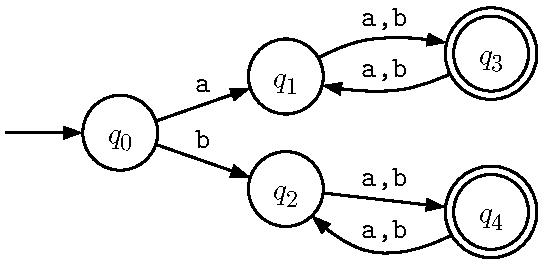
\includegraphics[scale=0.8]{Abbildungen/nicht-gleichwertig.pdf}
   \caption{A \simtextsc{Dfa} with equivalent states.}
  \label{fig:nicht-gleichwertig.dot}
\end{figure}

In general, we can minimize a \simtextsc{Dfa} by identifying certain states.   
If we look for example at the \simtextsc{Dfa} shown in figure \ref{fig:nicht-gleichwertig.dot}, we can identify
the states $q_1$ and $q_2$ as well as $q_3$ and $q_4$ without changing the language of the \simtextsc{Dfa}.
The resulting \simtextsc{Dfa} is shown in Figure \ref{fig:gleichwertig.dot} on page
\pageref{fig:gleichwertig.dot}.
The central idea in minimizing a \simtextsc{Dfa} is that we compute those states which \textbf{must not} be
identified and consider all other states as equivalent.  States that must not be identified are called
\blue{separable states}.  This notion is defined next.

\begin{Definition}[Separable States]
Assume $F = \langle Q, \Sigma, \delta, q_0, A \rangle$ is a \simtextsc{Dfa}.
Two states $p_1,p_2 \in Q$ are called \blue{separable} \index{separable} if and only if there exists a string 
$s \in \Sigma^*$ such that either
\begin{enumerate}
\item $\delta^*(p_1,s) \in    A$ and $\delta^*(p_2,s) \notin A$ or
\item $\delta^*(p_1,s) \notin A$ and $\delta^*(p_2,s) \in    A$
\end{enumerate}
holds.  In this case, the string $s$ \blue{separates} \index{separates} the states $p_1$ and $p_2$. \eox
\end{Definition}
If two states $p_1$ and $p_2$ are separable, then these states must not be identified since doing
so would change the language that is accepted.  We define an equivalence relation $\sim$ on the set $Q$ of all
states by setting 
\\[0.2cm]
\hspace*{1.3cm}
$p_1 \sim p_2$ \quad iff \quad 
$\forall s \in \Sigma^*:\bigl(\delta^*(p_1,s) \in A \leftrightarrow \delta^*(p_2,s) \in A\bigr)$.
\\[0.2cm]
Hence, two states $p_1$ and $p_2$ are considered to be equivalent iff they are not separable.   
The claim is that we can identify all pairs $\langle p_1, p_2\rangle$ of equivalent states.  

The question remains how we can determine which states are separable.
One possibility is to create a set $V \subseteq Q \times Q$ with pairs of states.  We add the pair $\langle p, q \rangle$ to the set
$V$ if we have discovered that $p$ and $q$ are separable.  We recognize $p$ and $q$ as separable if
there is a letter $c\in\Sigma$ and two states $s$ and $t$ that are already known to be separable such that 
\\[0.2cm]
\hspace*{1.3cm}
$\delta(p,c) = s$, \quad $\delta(q,c) = t$, \quad and \quad $\langle s, t \rangle \in V$
\\[0.2cm]
holds.  Formally, we define a sequence $(V_k)_{k\in\mathbb{N}}$ of sets of pairs of separable states by
induction.
\begin{enumerate}
\item[I.A.:] $k=0$

     Since an accepting state can never be equivalent to a non-accepting state we define
     \\[0.2cm]
     \hspace*{1.3cm}
     $V_0 := \bigl(A \times (Q \backslash A)\bigr) \cup \bigl((Q \backslash A) \times A\bigr)$.
     \\[0.2cm]
     Therefore, initially only the accepting states are separable from the states that are not accepting.
\item[I.S.:] $k \mapsto k + 1$

     If we have a pair $\pair(p,q) \in Q \times Q$ and a letter $c$ such that 
     the pair of states  $\langle \delta(p,c), \delta(q,c) \rangle$ is already separable, then $\langle p, q \rangle$ is
     separable, too.  Therefore we define:  
     \\[0.2cm]
     \hspace*{1.3cm}
     $V_{k+1} := V_k \cup \bigl\{ \pair(p,q) \bigm| \exists c \in \Sigma: \langle \delta(p,c), \delta(q,c) \rangle \in V_k \bigr\}$
\end{enumerate}
The sequence $(V_k)_{k\in\mathbb{N}}$ is monotonically increasing, i.e.~we have
\\[0.2cm]
\hspace*{1.3cm}
$V_{k} \subseteq V_{k+1}$.
\\[0.2cm]
Since $V_k \subseteq Q \times Q$ and the set $Q \times Q$ is finite, there must be a $K \in \mathbb{N}$ such that
\\[0.2cm]
\hspace*{1.3cm}
$V_{K+1} = V_K$.
\\[0.2cm]
We can therefore define two states $p$ and $q$ to be equivalent iff $\pair(p,q) \not\in V_K$:
\\[0.2cm]
\hspace*{1.3cm}
$p \sim q \; \stackrel{\mathrm{def}}{\Longleftrightarrow} \; \pair(p,q) \not\in V_K$.
\\[0.2cm]
Next, for a state $p \in Q$ we define the \blue{equivalence class} of $p$ as the set
\\[0.2cm]
\hspace*{1.3cm}
$[p]_\sim := \{ q \in Q \mid p \sim q \}$.
\\[0.2cm]
We define the set $\mathcal{Q}_\sim$ of all equivalence classes as
\\[0.2cm]
\hspace*{1.3cm}
$\mathcal{Q}_\sim := \bigl\{ [q]_\sim \bigm| q \in Q \bigr\}$.
\\[0.2cm]
Next, we define the function $\Delta: \mathcal{Q}_\sim \times \Sigma \rightarrow \mathcal{Q}_\sim$ as follows:
\\[0.2cm]
\hspace*{1.3cm}
$\Delta\bigl([q]_\sim, c\bigr) := \bigl[ \delta(q, c) \bigr]_\sim$.
\\[0.2cm]
Finally, we define the set of accepting equivalence classes $\widehat{A}$ as
\\[0.2cm]
\hspace*{1.3cm}
$\widehat{A} := \bigl\{ [q]_\sim \bigm| q \in A \bigr\}$.
\\[0.2cm]
Then, the \simtextsc{Dfa}
\\[0.2cm]
\hspace*{1.3cm}
$\mathtt{Min}(F) := \bigl\langle \mathcal{Q}_\sim, \Sigma, \Delta, [q_0]_\sim, \widehat{A} \bigr\rangle$
\\[0.2cm]
is the minimal complete \simtextsc{Dfa} that accepts the same language as the \simtextsc{Dfa} $F$.

\exampleEng
We consider the  \simtextsc{Dfa} shown in figure \ref{fig:nicht-gleichwertig.dot} and apply the algorithm
described above to this \simtextsc{Dfa}. 
We use a table for this.  The columns and rows of this table are numbered with the different states.  If we
have recognized in the first step that the states $i$ and $j$ are separable, we insert a $1$ in this
table in the $i$-th row and the $j$-th column. 
Furthermore, since the states $i$ and $j$ can also be distinguished from the states $j$ and $i$, we also insert
a $1$ in the $j$-th row and the $i$-th column.
As every state is equivalent to itself, the diagonal of the table is marked with $\sim$ from the beginning.
\begin{enumerate}
\item In the first step we recognize that the two accepting states $q_3$ and $q_4$ are separable from all non-accepting states.
      Therefore the pairs 
      $\pair(q_0,q_3)$,
      $\pair(q_0,q_4)$,
      $\pair(q_1,q_3)$,
      $\pair(q_1,q_4)$,
      $\pair(q_2,q_3)$ and
      $\pair(q_2,q_4)$
      are separable. Hence the table now has the following configuration:
      \begin{center}        
      \begin{tabular}[t]{|l||l|l|l|l|l|}
      \hline
            & $q_0$    &    $q_1$ &    $q_2$ &      $q_3$ &      $q_4$  \\
      \hline
      \hline
      $q_0$ & $\sim$   &          &          & $1$ & $1$  \\
      \hline
      $q_1$ &          & $\sim$   &          &$1$ &$1$  \\
      \hline
      $q_2$ &          &          & $\sim$   &$1$ &$1$  \\
      \hline
      $q_3$ &$1$        &$1$         &       $1$ & $\sim$   &           \\
      \hline
      $q_4$ &$1$ &$1$ &$1$ &          & $\sim$    \\
      \hline
      \end{tabular}
      \end{center}
\item Next we see that the states $q_0$ and $q_1$ are separable because
      \\[0.2cm]
      \hspace*{1.3cm}
      $\delta(q_0,a) = q_1$, \quad $\delta(q_1,a) = q_3$ \quad and \quad $q_1 \not\sim q_3$.
      \\[0.2cm]
      Also we see that the states $q_0$ and $q_2$ are separable, because
      \\[0.2cm]
      \hspace*{1.3cm}
      $\delta(q_0,b) = q_2$, \quad $\delta(q_2,b) = q_4$ \quad and \quad $q_2 \not\sim q_4$.
      \\[0.2cm]
      Since we have found in the second step that $q_0 \not\sim q_1$ and $q_0 \not\sim q_2$ hold true, we will insert a $2$ at the corresponding positions in the table. Therefore the table now has the following form:
      \begin{center}        
      \begin{tabular}[t]{|l||l|l|l|l|l|}
      \hline
        & $q_0$      &      $q_1$ &      $q_2$ &      $q_3$ &      $q_4$  \\
      \hline
      \hline
      $q_0$ & $\sim$   &$2$ &$2$ &$1$ &$1$  \\
      \hline
      $q_1$ &$2$ & $\sim$   &          &$1$ &$1$  \\
      \hline
      $q_2$ &$2$ &          & $\sim$   &$1$ &$1$  \\
      \hline
      $q_3$ &$1$ &$1$ &$1$ & $\sim$   &           \\
      \hline
      $q_4$ &$1$ &$1$ &$1$ &          & $\sim$    \\
      \hline
      \end{tabular}
      \end{center}
\item Now we do not find any more pairs of separable states, because if we take a look at the pair $\pair(q_1,q_2)$ we can see that
      \\[0.2cm]
      \hspace*{1.3cm}
      $\delta(q_1,\texttt{a}) = q_3$ \quad and \quad $\delta(q_2,\texttt{a}) = q_4$, 
      \\[0.2cm]
      but because the states $q_3$ and $q_4$ are not separable so far, this does not yield a new
      separable pair.  Neither does 
      \\[0.2cm]
      \hspace*{1.3cm}
      $\delta(q_1,\texttt{b}) = q_3$ \quad and \quad $\delta(q_2,\texttt{b}) = q_4$
      \\[0.2cm]
      yield a new separable pair.  At this point, the two states $q_3$ and $q_4$ remain.  We find
      \\[0.2cm]
      \hspace*{1.3cm}
      $\delta(q_3,c) = q_1$ \quad and \quad $\delta(q_4,c) = q_2$ \quad for all $c \in \{\texttt{a}, \texttt{b}\}$
      \\[0.2cm]
      and because the states $q_1$ and $q_2$ are not yet known to be separable, we have not found any new
      separable states.  Therefore, we can complete the table as shown below:

            \begin{center}        
      \begin{tabular}[t]{|l||l|l|l|l|l|}
      \hline
        & $q_0$      &      $q_1$ &      $q_2$ &      $q_3$ &      $q_4$  \\
      \hline
      \hline
      $q_0$ & $\sim$ &        $2$ &$2$ &$1$ &$1$  \\
      \hline
      $q_1$ &$2$ &  $\sim$        & $\sim$         &$1$ &$1$  \\
      \hline
      $q_2$ &$2$ &  $\sim$        & $\sim$         &$1$ &$1$  \\
      \hline
      $q_3$ &$1$ &$1$ &$1$ &  $\sim$ & $\sim$          \\
      \hline
      $q_4$ &$1$ &$1$ &$1$ &  $\sim$ & $\sim$          \\
      \hline
      \end{tabular}
      \end{center}

      Next, we read the equivalent states from the table and see that:
      \begin{enumerate}
      \item $q_1 \sim q_2$,
      \item $q_3 \sim q_4$.
      \end{enumerate}
      
      Figure \ref{fig:gleichwertig.dot} shows the corresponding reduced finite \simtextsc{Dfa}.
\end{enumerate}

\begin{figure}[!ht]
  \centering
  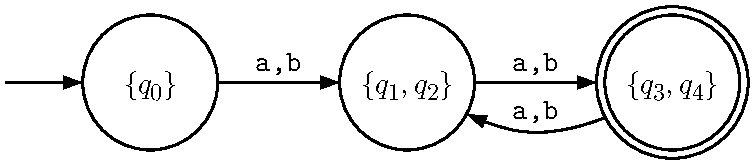
\includegraphics[scale=0.8]{Abbildungen/gleichwertig.pdf}
   \caption{The reduced \simtextsc{Dfa}.}
  \label{fig:gleichwertig.dot}
\end{figure}



\exerciseEng
Construct the minimal  \simtextsc{Dfa} that recognizes the language 
$L\bigl(a \cdot (b \cdot a)^*\bigr)$.  Perform the following steps:
\begin{enumerate}[(a)]
\item Construct an \simtextsc{Nfa} which recognizes this language.
\item Transform this \simtextsc{Nfa} into a  \simtextsc{Dfa}.
\item Minimize the number of states of this \simtextsc{Dfa} with the algorithm given above.
\end{enumerate}

\subsection{Implementation}
The \textsl{Jupyter notebook} 
\\[0.2cm]
\hspace*{1.3cm}
\href{https://github.com/karlstroetmann/Formal-Languages/blob/master/Python/Chapter-04-05/07-Minimize.ipynb}{\texttt{Python/Chapter-04-05/07-Minimize.ipynb}}
\\[0.2cm]
contains a program that takes a  \simtextsc{Dfa} $F$ and returns an equivalent \simtextsc{Dfa} that has
the minimum number of states.  It represents \simtextsc{Dfa}s with the types \texttt{TransRel} and \texttt{DFA} shown
in Figure \ref{fig:01-NFA-2-DFA.ipynb:types} on page \pageref{fig:01-NFA-2-DFA.ipynb:types}.  The states of
$\texttt{Min}(F)$ are equivalence classes, i.e.~sets of states of $F$.  For the reasons given in the discussion of
the function \texttt{bigUnion} in Section \ref{section:nfa-2-dfa}, they are represented as \texttt{frozenset}s.

\begin{figure}[!ht]
\centering
\begin{minted}[ frame         = lines,
                framesep      = 0.3cm,
                firstnumber   = 1,
                bgcolor       = sepia,
                numbers       = left,
                numbersep     = 0.3cm,
                xleftmargin   = 0.5cm,
                xrightmargin  = 0.5cm,
                gobble        = 4,
              ]{python3}
    def arb(M):
        x, *_ = M
        return x

    def cart_prod(A, B):
        return { (x, y) for x in A for y in B }

    def separate(Pairs, States, Σ, 𝛿):
        Result = { (q1, q2) for q1 in States
                            for q2 in States
                            for c  in Σ
                            if (𝛿[q1, c], 𝛿[q2, c]) in Pairs
                 }
        return Result

    def find_equivalence_class(p, Partition):
        return arb({ C for C in Partition if p in C })
\end{minted}
\vspace*{-0.3cm}
\caption{The functions \texttt{arb}, \texttt{cart\_prod}, \texttt{separate}, and \texttt{find\_equivalence\_class}.}
\label{fig:07-Minimize.ipynb:separate}
\end{figure}

\noindent
Figure \ref{fig:07-Minimize.ipynb:separate} on page \pageref{fig:07-Minimize.ipynb:separate} shows some auxiliary
functions.
\begin{enumerate}
\item Line 1 -- 3 define the function \texttt{arb}, which returns an arbitrary element of a non-empty set $M$.
      The assignment in line 2 assigns the first element that is found when the elements of $M$ are enumerated to
      the variable \texttt{x}, while the variable \texttt{\_} collects the remaining elements, which are not
      used.
\item Line 5 -- 6 define the function \texttt{cart\_prod}, which computes the Cartesian product
      $A \times B = \bigl\{ \pair(x, y) \bigm| x \in A \wedge y \in B \bigr\}$.
\item Line 8 -- 14 define the function \texttt{separate}.  Given a set \texttt{Pairs} of pairs of states that are
      known to be separable, it computes the set
      \\[0.2cm]
      \hspace*{1.3cm}
      $\bigl\{ \pair(p,q) \bigm| \exists c \in \Sigma: \langle \delta(p,c), \delta(q,c) \rangle \in \texttt{Pairs}
      \bigr\}$
      \\[0.2cm]
      of all pairs that are separable because of these pairs.  Here, the transition function \texttt{𝛿} has to
      be complete, since otherwise the expression \texttt{𝛿[q1, c]} fails for a missing key.
\item Line 16 -- 17 define the function \texttt{find\_equivalence\_class}.  Given a state $p$ and a partition of
      the set of states, i.e.~a set of disjoint sets that cover all states, it returns the set $C$ of the
      partition that contains $p$:  The set comprehension in line 17 yields the set $\{ C \}$, and the function
      \texttt{arb} extracts its only element.
\end{enumerate}

\begin{figure}[!ht]
\centering
\begin{minted}[ frame         = lines,
                framesep      = 0.3cm,
                firstnumber   = 1,
                bgcolor       = sepia,
                numbers       = left,
                numbersep     = 0.3cm,
                xleftmargin   = 0.5cm,
                xrightmargin  = 0.5cm,
                gobble        = 4,
              ]{python3}
    def all_separable_step(S, Q, Σ, 𝛿):
        return S | separate(S, Q, Σ, 𝛿)

    def all_separable(Q, A, Σ, 𝛿):
        Separable = cart_prod(Q - A, A) | cart_prod(A, Q - A)
        return fixpoint(all_separable_step, Separable, Q, Σ, 𝛿)

    def reachable_step(R, Σ, 𝛿):
        return R | { 𝛿[p, c] for p in R for c in Σ }

    def reachable(q0, Σ, 𝛿):
        return fixpoint(reachable_step, { q0 }, Σ, 𝛿)
\end{minted}
\vspace*{-0.3cm}
\caption{The functions that compute the separable pairs and the reachable states.}
\label{fig:07-Minimize.ipynb:all_separable}
\end{figure}

\noindent
Figure \ref{fig:07-Minimize.ipynb:all_separable} on page \pageref{fig:07-Minimize.ipynb:all_separable} shows the
functions that compute the set of all separable pairs and the set of all reachable states.  Both sets are computed
by a fixpoint iteration.  The notebook contains a copy of the function \texttt{fixpoint} that is shown in Figure
\ref{fig:01-NFA-2-DFA.ipynb:fixpoint} on page \pageref{fig:01-NFA-2-DFA.ipynb:fixpoint}.
\begin{enumerate}
\item Line 1 -- 2 define the function \texttt{all\_separable\_step}, which computes the step from $V_k$ to
      $V_{k+1}$ in the definition of the sets $V_k$ given above, since we have
      \\[0.2cm]
      \hspace*{1.3cm}
      $\begin{array}[t]{lcl}
       V_{k+1} & = & V_k \cup \bigl\{ \pair(p,q) \bigm| \exists c \in \Sigma: \langle \delta(p,c), \delta(q,c)
                     \rangle \in V_k \bigr\} \\[0.1cm]
               & = & \texttt{all\_separable\_step}(V_k, Q, \Sigma, \delta).
       \end{array}$
\item Line 4 -- 6 define the function \texttt{all\_separable}.  Line 5 computes the set
      $V_0 = \bigl(A \times (Q \backslash A)\bigr) \cup \bigl((Q \backslash A) \times A\bigr)$.  For sets, the
      operator ``\texttt{-}'' computes the difference.  Starting with $V_0$, the fixpoint iteration in line 6
      computes the sets $V_1$, $V_2$, $\cdots$ until it finds a set $V_K$ such that $V_{K+1} = V_K$.  This set
      contains all pairs of separable states.
\item Line 8 -- 9 define the function \texttt{reachable\_step}.  The set of all states that are reachable from the
      start state $q_0$ is the smallest set $R$ such that $q_0 \in R$ holds and such that $R$ is a fixpoint of
      the function
      \\[0.2cm]
      \hspace*{1.3cm}
      $\textsl{reachable\_step}(R) := R \cup \bigl\{ \delta(p, c) \bigm| p \in R \wedge c \in \Sigma \bigr\}$.
\item Line 11 -- 12 define the function \texttt{reachable}.  Like the function \texttt{allStates} in Figure
      \ref{fig:01-NFA-2-DFA.ipynb:fixpoint}, it computes this set with a fixpoint iteration that starts with the
      set $\{ q_0 \}$.  After $n$ steps, the set contains exactly those states that can be reached from $q_0$ by
      reading at most $n$ characters.
\end{enumerate}

\begin{figure}[!ht]
\centering
\begin{minted}[ frame         = lines,
                framesep      = 0.3cm,
                firstnumber   = 1,
                bgcolor       = sepia,
                numbers       = left,
                numbersep     = 0.3cm,
                xleftmargin   = 0.5cm,
                xrightmargin  = 0.5cm,
                gobble        = 4,
              ]{python3}
    def minimize(F):
        Q, Σ, 𝛿, q0, A = F
        Q              = reachable(q0, Σ, 𝛿)
        Separable      = all_separable(Q, A, Σ, 𝛿)
        Equivalent     = cart_prod(Q, Q) - Separable
        EquivClasses   = { frozenset({ p for p in Q
                                         if (p, q) in Equivalent })
                           for q in Q
                         }
        newQ0          = arb({ M for M in EquivClasses if q0 in M })
        newAccept      = { M for M in EquivClasses if arb(M) in A }
        newDelta = {}
        for q in Q:
            classOfQ = find_equivalence_class(q, EquivClasses)
            for c in Σ:
                newDelta[(classOfQ, c)] = find_equivalence_class(
                                              𝛿[q, c], EquivClasses)
        return EquivClasses, Σ, newDelta, newQ0, newAccept
\end{minted}
\vspace*{-0.3cm}
\caption{The function \texttt{minimize}.}
\label{fig:07-Minimize.ipynb:minimize}
\end{figure}

\noindent
Figure \ref{fig:07-Minimize.ipynb:minimize} on page \pageref{fig:07-Minimize.ipynb:minimize} shows the function
\texttt{minimize}, which computes $\texttt{Min}(F)$ for a complete \simtextsc{Dfa} $F$.
\begin{enumerate}
\item Line 2 extracts the components of $F$.
\item Line 3 replaces the set of states by the set of reachable states.  The theory has assumed that all states
      of $F$ are reachable.  This line ensures that this assumption is satisfied.
\item Line 4 computes the set $V_K$ of all pairs of separable states, and line 5 computes the equivalence relation
      $\sim$ as the set of all pairs of states that are not separable.
\item Line 6 -- 9 compute the set $\mathcal{Q}_\sim = \bigl\{ [q]_\sim \bigm| q \in Q \bigr\}$ of all equivalence
      classes, where $[q]_\sim = \{ p \in Q \mid p \sim q \}$.  Equivalent states have the same equivalence class.
      As \texttt{EquivClasses} is a set, it contains every equivalence class only once.
\item Line 10 computes the start state $[q_0]_\sim$ of $\texttt{Min}(F)$, which is the equivalence class that
      contains $q_0$.
\item Line 11 computes the set $\widehat{A} = \bigl\{ [q]_\sim \bigm| q \in A \bigr\}$ of accepting states.  It
      checks whether an arbitrary element of an equivalence class $M$ is accepting.  This is sufficient, since an
      accepting state and a state that is not accepting are separable by the empty string.  Hence an equivalence
      class contains either only accepting states or no accepting state at all.
\item Line 12 -- 17 compute the transition function
      $\Delta\bigl([q]_\sim, c\bigr) = \bigl[ \delta(q, c) \bigr]_\sim$.  If an equivalence class contains several
      states, its transitions are computed once for each of them.  All these computations yield the same
      result:  If $p \sim q$, then $\delta(p, c) \sim \delta(q, c)$, since otherwise the pair $\pair(p,q)$ would
      be separable.
\item Line 18 returns the five components of $\texttt{Min}(F)$.
\end{enumerate}
The notebook
\href{https://github.com/karlstroetmann/Formal-Languages/blob/master/Python/Chapter-04-05/08-Test-Minimize.ipynb}{\texttt{08-Test-Minimize.ipynb}}
minimizes a \simtextsc{Dfa} with nine states and draws both finite state machines.

The \textsl{Jupyter notebook}
\\[0.2cm]
\hspace*{1.3cm}
\href{https://github.com/karlstroetmann/Formal-Languages/blob/master/Python/Chapter-04-05/07-Minimize-Table.ipynb}{\texttt{Python/Chapter-04-05/07-Minimize-Table.ipynb}}
\\[0.2cm]
implements the same algorithm, but it also computes the tables that have been used in the example above
and displays them.  For every step, it explains why the pairs of states that are entered into the table
are separable.  Besides the example discussed above, this notebook minimizes a \simtextsc{Dfa} with eight
states that accepts all strings ending with \texttt{abb}.


\section{Conclusion}
In this chapter we have shown that the concept of a \blue{finite state machine}
and the concept of a \blue{regular expression} are equivalent in their ability to describe formal languages.
\begin{enumerate}[(a)]
\item Every \simtextsc{Dfa} can be translated into an equivalent regular expression.
\item Every regular expression can be translated into an equivalent \simtextsc{Nfa}.
\item Every \simtextsc{Nfa} can be transformed into an equivalent \simtextsc{Dfa}.
\end{enumerate}
Furthermore, we have shown that every \simtextsc{Dfa} can be minimized.

\paragraph{Historical Remark}
\href{http://en.wikipedia.org/wiki/Stephen_Cole_Kleene}{Stephen Cole Kleene} (1909 -- 1994) has shown in 1956 that the concepts of 
\blue{finite state machines} and \blue{regular expressions} have the same strength
\cite{kleene:1956}.

\section{Check Your Understanding}
\begin{enumerate}[(a)]
\item How are \simtextsc{Dfa}s and \simtextsc{Nfa}s defined?
\item Given an \simtextsc{Nfa} $F$, can you convert it into an equivalent \simtextsc{Dfa}
      $\textsl{det}(F)$ that accepts the same language as the \simtextsc{Nfa} $F$?
\item Given a regular expression $r$, can you describe the steps necessary to construct an 
      \simtextsc{Nfa} $F$ that accepts the language specified by $r$?
\item Given a \simtextsc{Dfa} $F$ can you describe how to construct a regular expression $r$
      that specifies the language accepted by $F$?
\item How do we minimize a \simtextsc{Dfa}?
\end{enumerate}

%%% Local Variables: 
%%% mode: latex
%%% TeX-master: "formal-languages.tex"
%%% End: 
